\chapter{模式构架}\label{模式构架}
%\addcontentsline{toc}{chapter}{模式结构}
\section{网格构建}\label{网格构建}
\begin{mymdframed}{代码}
本节对应的网格类型可在\texttt{/include/define.h}中进行选择。
\end{mymdframed}

通用陆面模式(CoLM,the Common Land Model)首先对陆地表面进行剖分,将模拟区域按一定规则划分成单元(Element),模拟分辨率决定了单元平均面积的大小。CoLM中包含三种单元划分规则:1)经纬度网格(图~\ref{fig:经纬度网格});2)非结构网格(三角形/六边形)(图~\ref{fig:六边形单元网格},~\ref{fig:三角形单元网格});3)流域单元(Catchment)(图~\ref{fig:流域单元网格})。除默认的三种网格外,CoLM实际可使用任意形状单元的网格。

{
\begin{figure}[htbp]
\centering
\includegraphics[width=0.8\textwidth]{Figures/模式构架/网格-格点.jpg}
\caption{CoLM中可使用的网格(1):经纬度单元}
\label{fig:经纬度网格}
\end{figure}
}
{
\begin{figure}[htbp]
\centering
\includegraphics[width=0.8\textwidth]{Figures/模式构架/网格-六边形.jpg}
\caption{CoLM中可使用的网格(2):六边形单元}
\label{fig:六边形单元网格}
\end{figure}
}
 {
\begin{figure}[htbp]
\centering
\includegraphics[width=0.8\textwidth]{Figures/模式构架/网格-三角形.jpg}
\caption{CoLM中可使用的网格(3):三角形单元}
\label{fig:三角形单元网格}
\end{figure}
}
 {
\begin{figure}[htbp]
\centering
\includegraphics[width=0.8\textwidth]{Figures/模式构架/网格-流域.jpg}
\caption{CoLM中可使用的网格(4):流域单元网格}
\label{fig:流域单元网格}
\end{figure}
}

\subsection{经纬度网格}\label{经纬度网格}
经纬度网格通过规定经度和纬度分割线的位置来建立,单元的边界由东西两段经线和南北两段纬线组成。经纬度网格的分辨率通常使用经纬度分割线的间距来表达,例如,分辨率为0.5\textdegree 表示相邻两条纬度分割线和经度分割线的距离均为0.5\textdegree。经度分割线和纬度分割线分别可以是不等间距的,当间距不等时,需从外部数据读入分割线的位置来定义模拟区域的经纬度网格。

\subsection{非结构网格}\label{非结构网格}
在原有的经纬度网格基础上,CoLM 新开发了一个非结构化网格构建工具,它可以基于多个水平分布特征,自动识别不同区域所需的网格分辨率,生成包括三角形网格和多边形网格(以六边形网格为主)在内的无规则拓扑关系网格。具体而言,非结构网格的分辨率取决于所指定的一个或者多个目标的分布特征(例如高程、坡度、土地利用、植被类型等)。该工具可在目标变化梯度较大的地区采用高分辨率,在变化梯度较小的地区采用低分辨率。因此基于非结构化网格的多分辨率模拟保留了全局模型的整体结构,同时支持局部区域的高分辨率模拟。

在非结构网格的构建过程中,该工具首先基于 Delaunay 三角网等值线生成算法构建初始网格,即将经纬度网格数据转化插值,生成铺盖整个球面的三角形网格数据;接着根据所选取的目标进行一次或者多次细化与网格结构调整;再依次连接具有相同顶点的五至七个三角形重心生成多边形网格,最后输出全球区域的三角形或多边形可变分辨率网格。总之,非结构网格具有灵活性强、节点和单元的分布可控性好、能较好地控制网格的大小和节点的密度等优点。模式运行流程如图~\ref{fig:非结构化网格CoLM总体运行流程图} 所示。

{
\begin{figure}[htbp]
\centering
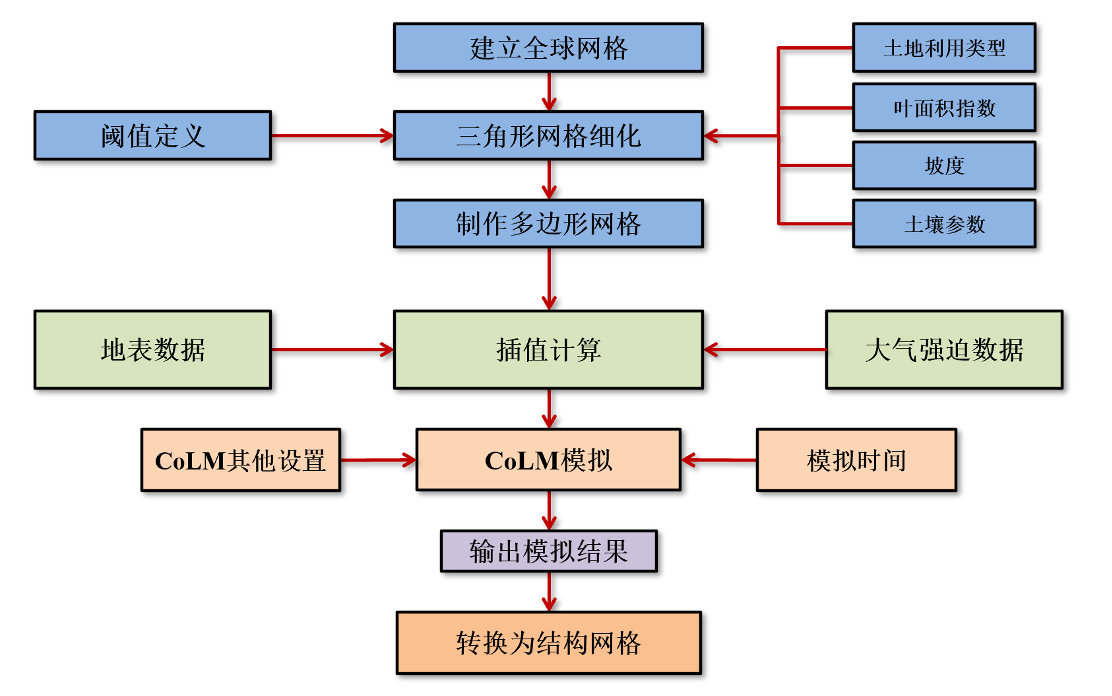
\includegraphics[width=0.8\textwidth]{Figures/模式构架/非结构化网格CoLM总体运行流程图.png}
\caption{非结构化网格CoLM总体运行流程图}
\label{fig:非结构化网格CoLM总体运行流程图}
\end{figure}
}

该工具基于非结构化一致性三角-六边形构建算法 \citep{fatichi2020soil,walko2008ocean,walko_direct_2011},以准均匀的全局三角形(Delaunay)的网格化方法为理论依据。其中非结构网格构造流程如图~\ref{fig:非结构化网格生成流程图} 所示,具体介绍如下:
{
\begin{figure}[htbp]
\centering
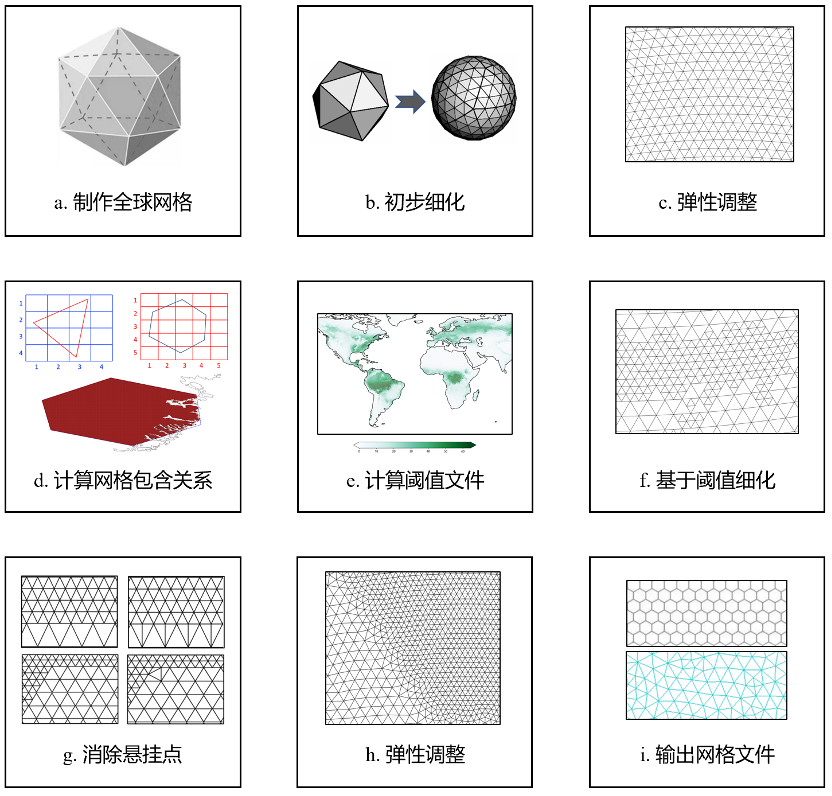
\includegraphics[width=\textwidth]{Figures/模式构架/非结构化网格生成流程图.png}
\caption{非结构化网格生成流程图}
\label{fig:非结构化网格生成流程图}
\end{figure}
}

{
\begin{table}[htbp]
\centering
\caption{细化阈值文件}
\label{tab:细化阈值文件}
\begin{tabular}{@{}ll@{}}
\toprule
变量名            & 具体描述           \\\midrule
num\_landtypes & 网格包含的土地类型数量    \\
f\_mainland    & 网格主导土地类型       \\
max\_iter      & 三角形网格最大细化迭代次数  \\
lai            & 叶面积指数          \\
slope          & 坡度             \\
k\_s           & 饱和导水率          \\
k\_solids      & 土壤固体导热系数       \\
tkdry          & 土壤导热系数(干燥)     \\
tksatf         & 土壤导热系数(冻结、饱和)  \\
tksatu         & 土壤导热系数(未冻结、饱和) \\\bottomrule
\end{tabular}
\end{table}
}

{
\begin{figure}[htbp]
\centering
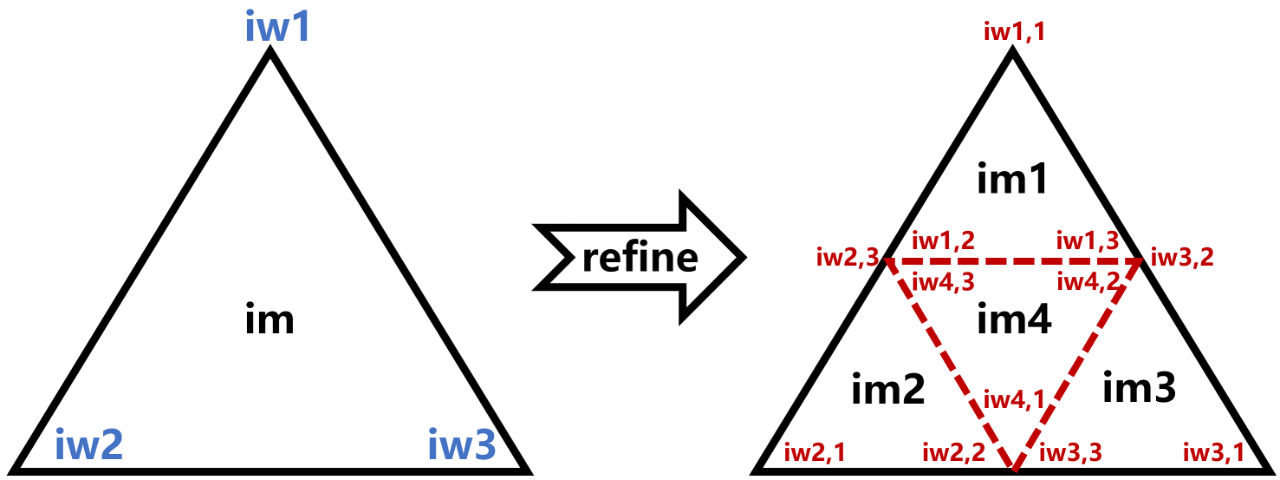
\includegraphics[width=\textwidth]{Figures/模式构架/三角形网格简易细化.png}
\caption{三角形网格简易细化}
\label{fig:三角形网格简易细化}
\end{figure}
}

\begin{enumerate}
\item 构建初始网格

在此过程中,首先将一个正二十面体投射到地球表面,它的12个顶点中有两个位于南北两极,其余的位于$\pm\arctan(1/2)$ 纬度。正二十面体网格的二维投影基于0\textdegree 经线所在经线圈与与0\textdegree 维度所在纬线圈轴对称。这有利于在计算包含关系时简化运算步骤。同时每个区域被划分为面积基本相同大小的三角形分块,以满足非结构网格初步细化和提升并行化计算效率的需要。

\item 初步细化

在此步骤中,网格生成工具能够将每个球面三角形面细分为NXP $\times$ NXP更小的三角形,其中NXP可设置为任意正整数,代表所选的网格分辨率。NXP定义为两个相邻多边形网格的水平网格间距(网格单元面积的平方根),网格的分辨率大约等于7200公里/NXP。因此,如果试图在网格上获得100公里的水平网格间距,应将NXP设置为“72”。这种网格配置采用基于二十面体改进的六边形或三角形网格单元的非结构化网格,从而避免了传统经纬度网格的南北极奇点。该网格配置为局部网格细化提供了一种完全无缝的自然适应性,不需要额外特殊的网格嵌套算法。

\item 弹簧动态调整

考虑到地球球面对三角形网格实际边长的影响,通过初步细化生成的三角形并不等同于等边三角形。\citet{tomita2002optimization}描述了一种称为“Spring Dynamics”的计算方法,用于在准均匀的全局网格上调整三角形网格单元的形状和大小。该方法代表了一种物理模拟,其中网格中的每个边都像弹簧一样在其顶点间施加吸引力或相反的力,该弹力取决于其自身的长度、平衡长度和弹簧系数。该研究表明,将平衡长度设置为使弹簧松弛在数值上稳定的最大可能值,即接近整个网格的平均边长,会产生最小的网格单元尺寸的空间变化,并且调整过程能显著提高模型的数值精度。

\item 计算包含关系

CoLM非结构网格的空间细分基于三角形网格与阈值数据(部分地表数据,如表~\ref{tab:细化阈值文件})进行。一般来说,三角形网格的分辨率远低于阈值数据集。这些高分辨率网格(以下简称像素)构成了非结构化网格。在进行网格细化之前,需要计算两者间的包含关系,并得到每个网格对应像素的索引,以便识别像素对非结构网格的归属。最后,根据这些像素的信息,用户可以了解特定网格内的空间异质性,并决定是否需要对其进行细化。这个过程将在细化过程中的每次迭代中执行。

\item 阈值文件计算


\citet{walko_direct_2011} 中的细化面积和程度是通过分配一系列点的经纬度坐标来确定的(例如,(lat = 30.1, lon = 120.5); \dots)加上影响半径(例如,(R = 1km); \dots)。与之不同,CoLM的网格细化工具能够根据各种指标确定精细化的区域。关于这些指标的详细信息可以在表~\ref{tab:细化阈值文件} 中找到。该工具允许对一个或多个网格进行细化,并约束到用户定义的阈值。换言之,CoLM 可以根据任意数量的重要特征对网格进行细化,例如 $LAI$ 的标准差,网格内土地利用类型数量等。图~\ref{fig:多阈值非结构网格细化} 展示了基于多种不同地表特征进行细化得到的全球陆面多边形网格。

{
\begin{figure}[htbp]
\centering
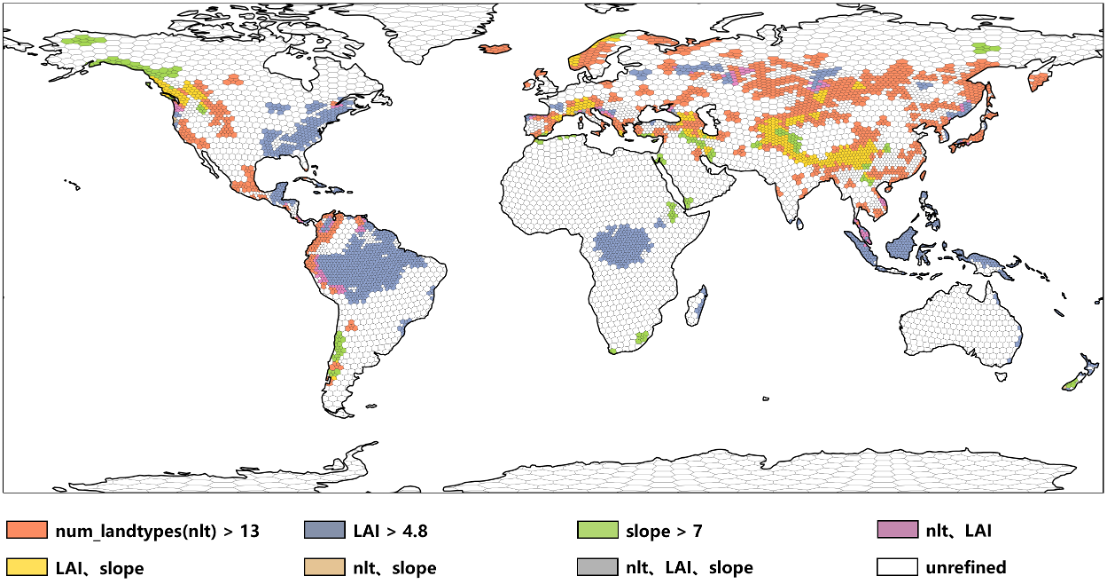
\includegraphics[width=\textwidth]{Figures/模式构架/多阈值非结构网格细化.png}
\caption{多阈值非结构网格细化示例}
\label{fig:多阈值非结构网格细化}
\end{figure}
}

\item 阈值细化

如图~\ref{fig:非结构化网格生成流程图} 所示,本步骤主要实现三角形网格的阈值细化。利用生成的初始三角形网格包含关系,可计算三角形网格下各阈值数组,再根据阈值标记网格是否需要细化。如图~\ref{fig:三角形网格简易细化} 所示,通过将三角形网格“分成四格”,即可提高三角形网格的分辨率。然后,将新生成的网格信息添加到原始数组中,并标记被细化的网格。在计算新生成网格的包含关系时,只需要遍历被细化三角形最小外围矩形内的经纬度网格,可以大大减少计算时间。当迭代次数超过阈值或所有三角形网格满足阈值时,阈值细化终止,程序将输出最终生成的带有包含信息的三角形网格信息数据(见表~\ref{tab:细化阈值文件})。图~\ref{fig:根据LAI对非结构网格进行多重细化} 展示了基于叶面积指数特征进行多层级细化所生成的多边形网格结构。

{
\begin{figure}[htbp]
\centering
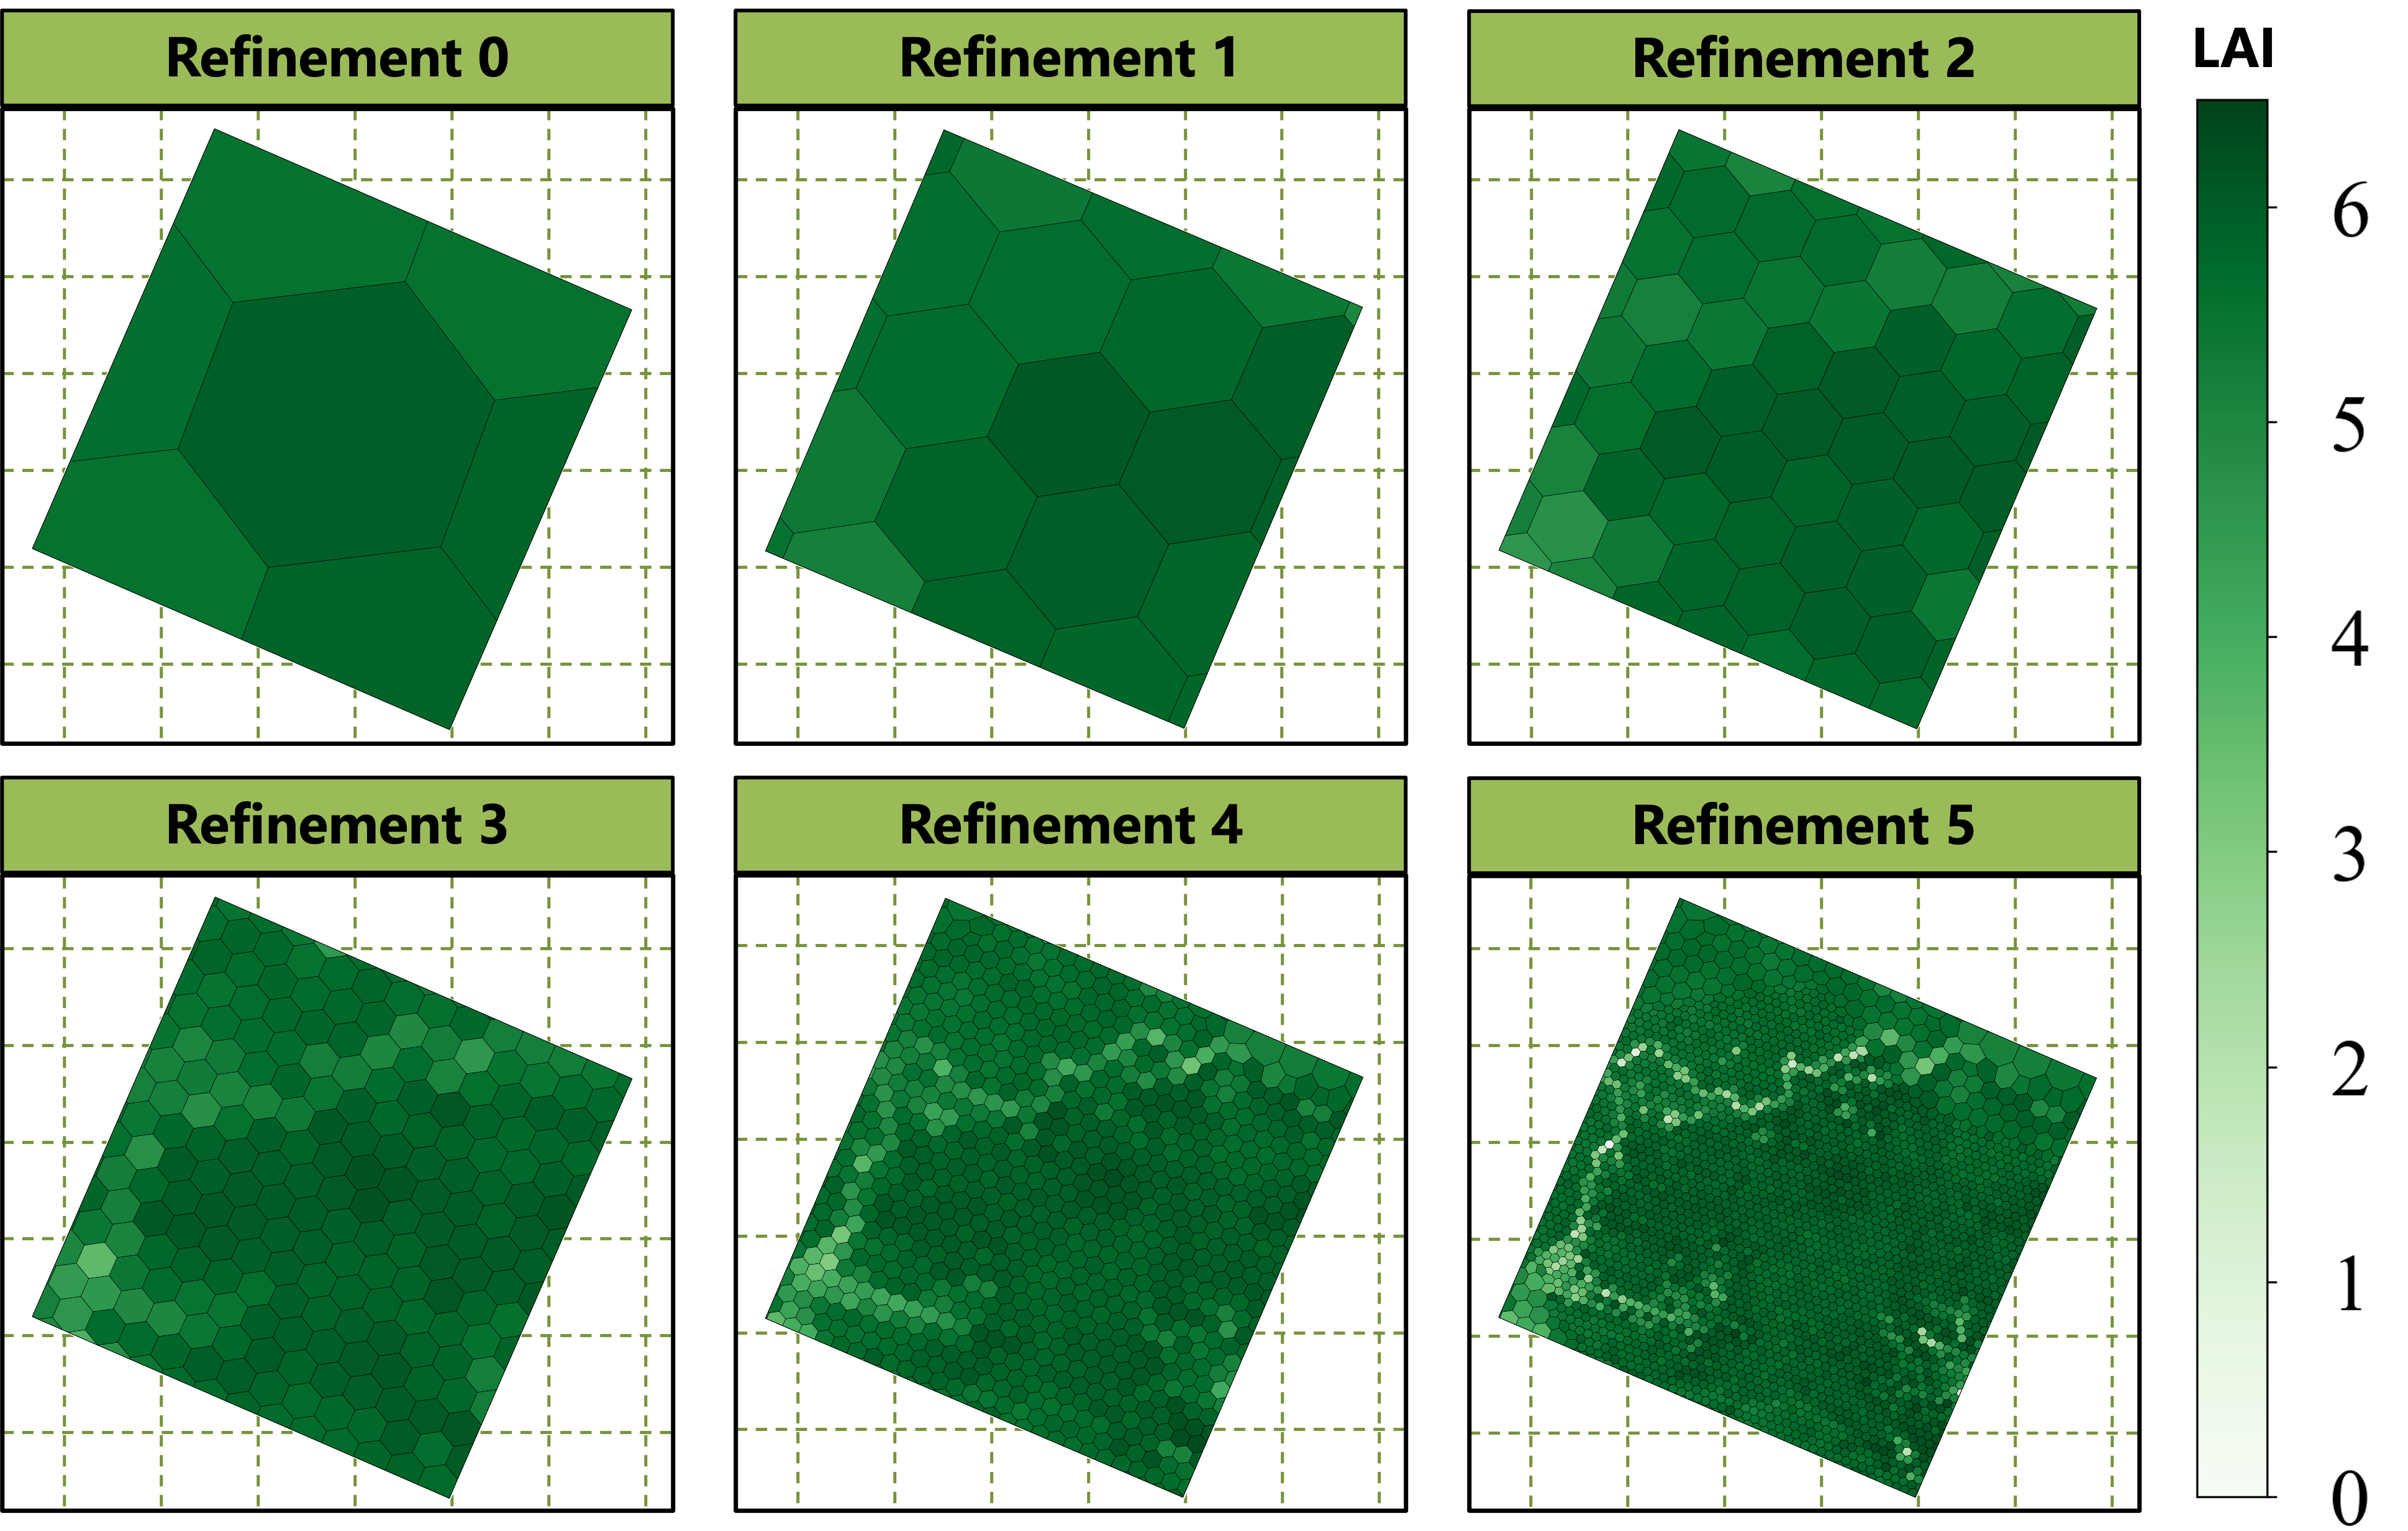
\includegraphics[width=0.8\textwidth]{Figures/模式构架/根据LAI对非结构网格进行多重细化.png}
\caption{根据LAI对非结构网格进行多重细化}
\label{fig:根据LAI对非结构网格进行多重细化}
\end{figure}
}

\item 清除悬挂点\\
该步骤将网格细化生成的附着在原始三角形边缘上的点称为悬挂点。为了保证每个三角形只与三个相邻三角形共享边,我们针对两种情况设置了不同的悬挂点消除方案。如图~\ref{fig:非结构化网格生成流程图} 顶部所示,对于细化边缘较平坦的区域,可以连接悬挂点与其相邻三角形的顶点。而对于一些凹陷区域,如图~\ref{fig:非结构化网格生成流程图} 底部所示,由于多个悬挂点位置相邻,直接连接悬挂点与其相邻三角形的顶点会使顶点被相邻的八条边共享,导致生成多边形网格时产生八边形,因此我们采用了特殊的细化方法来避免这一问题。此外,在消除悬挂点时,如果两个细化区域的边界相遇,也容易产生八边形。综上所述,在消除悬挂点前,需要对初步细化后的网格进行如下预处理:
\begin{enumerate}
\item 遍历所有未细化的三角网格。当其相邻的3个三角形网格中有1个以上被细化时,该三角形网格需要被细化。
\item 在三角形网格中找到并记录凹陷区域(即图~\ref{fig:非结构化网格生成流程图} 底部细化区域)。当两个凹陷区域有一个公共三角形网格时,细化组成它们的三个三角形网格
\item 循环遍历所有三角形网格顶点,计算剔除悬挂点后该点将添加的邻边数,当增加后其邻边数大于七时,细化其所有邻接三角形网格。在预处理过程中,三个进程依次进入迭代。当三个过程同时没有进行网格细化时,视为预处理完成。预处理完成后,可以进行消除悬挂点操作(即图~\ref{fig:非结构化网格生成流程图}),并得到可用于构建多边形网格的三角形网格。
\end{enumerate}
\item 网格调整和多边形网格生成\\
在消除悬挂点的操作过程中,消除凹陷区域会生成许多钝角三角形。而多边形网格由三角形网格重心连接而成,因此过多的钝角三角形会导致生成的部分多边形与正多边形偏差较大,进而降低网格的各向同性,最终影响网格在CoLM等水文模型中的应用。为了在不过度影响原有网格结构的情况下对网格进行校正,本文根据钝角三角形角度与边长计算经纬度位移分量,并对其进行迭代调整。当不存在钝角三角形或迭代次数超过阈值时,调整结束。在每次迭代过程中,通过三角形网格重心构造多边形网格,并计算三角形网格与正三角形、多边形网格与正多边形角度的标准差,这是衡量非结构网格自身各向同性的标准之一。在每次迭代过程中,通过三角网格的重心构造多边形网格,并计算三角形网格与正三角形、多边形网格与正多边形的标准差,这是衡量网格自身物理结构质量的标准之一。迭代完成后,通过三角网格重心所构造处的最后一个多边形网格即为最终结果。
\item 输出网格文件\\
在上述步骤完成之后,可输出两种类型的网格。一是最后一次迭代生成的三角形网格,二是根据前者重心连接构造的多边形网格。在 MPI 版本中,无需将地表、大气等初始数据的存储方式由经纬度网格转换为非结构化网格,就可以实现 CoLM 中地表水文过程在非结构化网格上的模拟。
\end{enumerate}


\subsection{流域单元网格}\label{流域单元网格}
流域单元为面积大致相同的集水区域(图~\ref{fig:流域单元网格})。流域单元考虑了网格单元之间的水文关联以及单元内部的水文结构,基于流域单元网格,可建立对产流和汇流动力学过程的模拟方案。此外,流域单元及其次级单元(高度带单元)的划分主要依赖高程数据,在陆面过程受地形影响较为显著的区域,采用流域单元网格可显著减少网格内陆表变量的异质性,提高模式模拟的精度。

CoLM中的流域单元网格为三级结构:第一级为流域单元,第二级为高度带单元,第三级为次网格单元(图~\ref{fig:流域单元示意图})。其中,流域单元和高度带单元使用水文学数据生成,次网格单元的生成方法与其他网格中的次网格单元相同(见~\ref{次网格}~节)。

{
\begin{figure}[htbp]
\centering
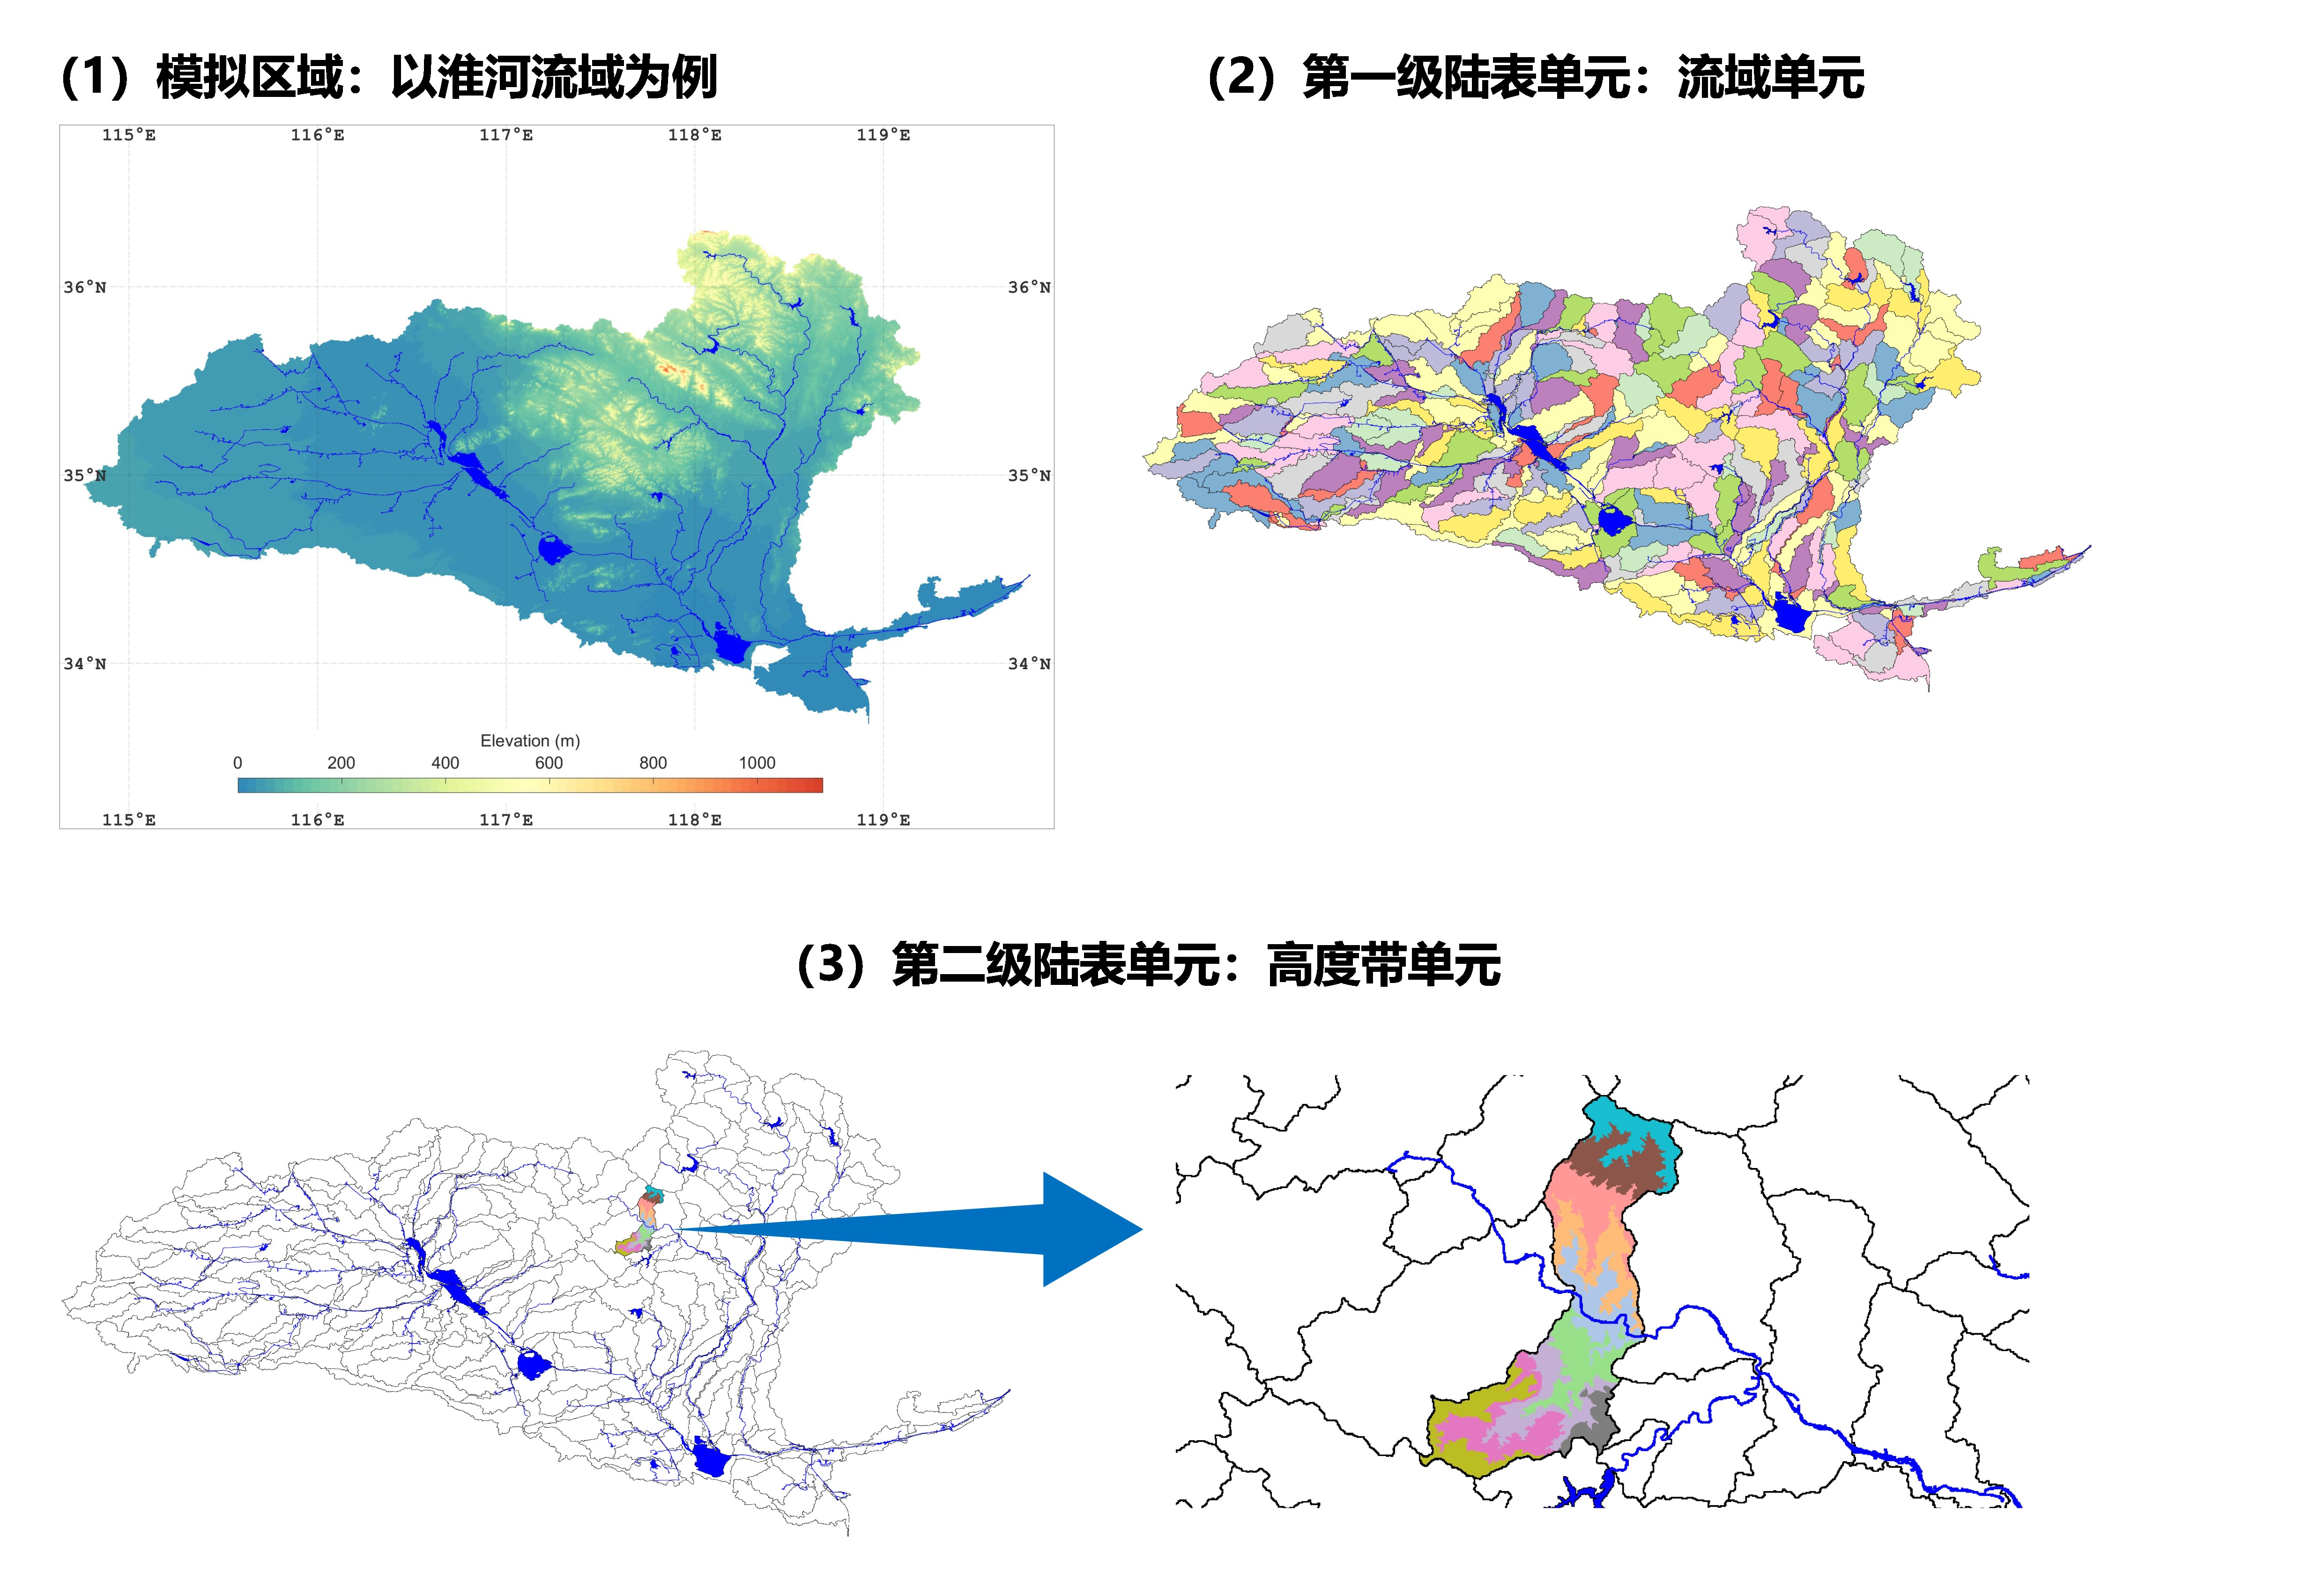
\includegraphics[width=\textwidth]{Figures/模式构架/流域单元示意图.jpg}
\caption{CoLM中的流域单元网格划分示意图}
\label{fig:流域单元示意图}
\end{figure}
}

流域单元(第一级)为面积大致相同的集水区域(图~\ref{fig:流域单元示意图}(2))。流域单元网格的分辨率表示为一个单元的面积阈值(即河道集水区域的面积阈值,记为Cat-size)。流域单元的划分使用高分辨率的“上游集水面积”(UPA)和“水流方向”格点数据(其中的格点以下称为像素点),分为两个步骤。
第一步,提取研究区域的河道像素点并将其分段。此处的河道像素点定义为上游集水面积大于或等于Cat-size的像素点,未必为真实的河道。提取完成后,根据以下三个规则从下游至上游将河道分段:1.一段河道内没有河道分支;2.局部集水面积(定义为该河段的总集水面积减去上游河道的集水面积)不超过Cat-size;3.河道长度小于Cat-size的平方根。其中,规则1的目的是排除汇流点在流域单元内部的情况,以更合理地进行汇流过程的模拟;规则3的目的是避免流域单元较为狭长,以减少单元内部陆表变量的变化。
第二步,根据河道分段将研究区域划分为流域单元。一个流域单元定义为一段河道的局部集水区域。对每个像素点,可根据水流方向数据向下找到其所在的流域单元。

高度带单元(第二级)为主要依赖高程进行划分的流域单元内部子区域(图~\ref{fig:流域单元示意图}(3))。因流域面积较大时,一段河道的上下游会有落差,CoLM中不直接使用高程数据对流域单元进行划分,而是使用像素点的排水高度。排水高度定义为一个像素点和它流入的河道点的高度差(Height above nearest drainage, HAND),可根据高程数据和像素点与河道的汇流关系计算得出。此外,为了基于高度带单元进行产流动力学过程的模拟,CoLM对高度带单元的划分进行了进一步的约束,划分后的高度带单元需满足:1)连通性;2)每个高度带单元都有唯一的下游单元。对高度带单元进行划分的算法见图~\ref{fig:高度带单元算法流程}。

{
\begin{figure}[htbp]
\centering
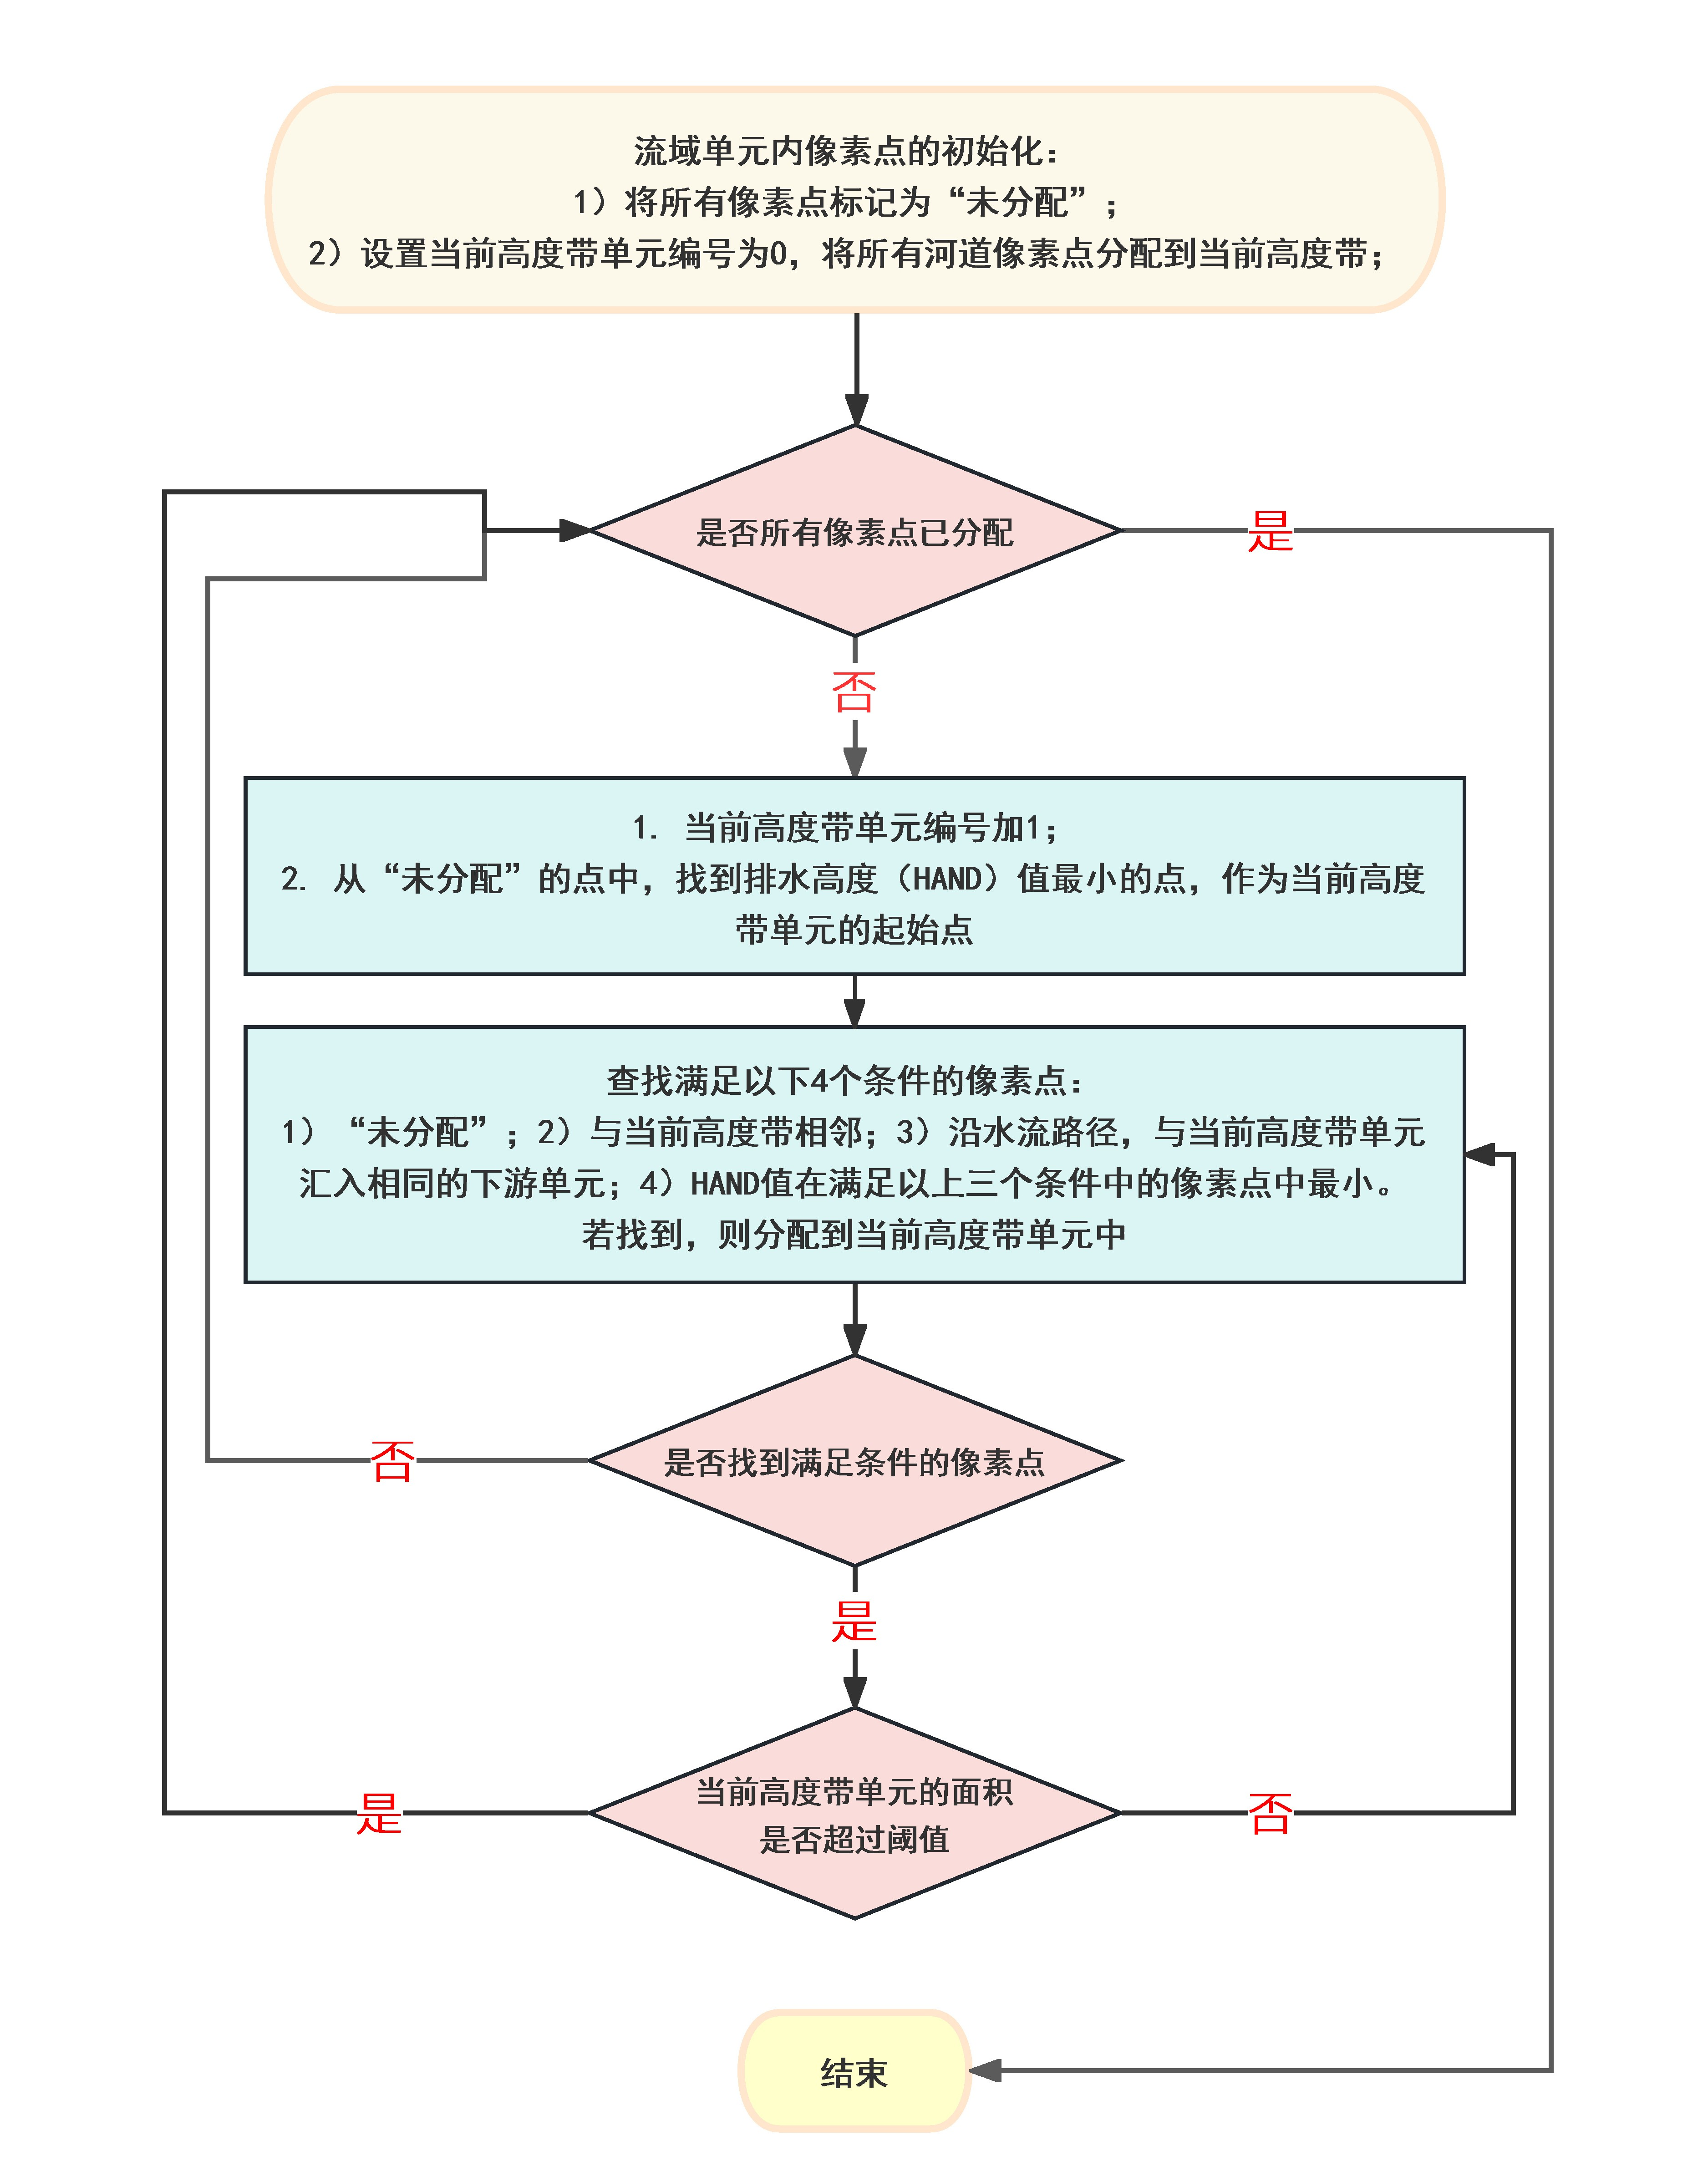
\includegraphics[width=0.8\textwidth]{Figures/模式构架/高度带单元划分算法.jpg}
\caption{高度带单元划分算法流程图}
\label{fig:高度带单元算法流程}
\end{figure}
}

图~\ref{fig:高度带单元约束示意}~显示了对高度带单元的划分进行上述约束的作用。仅使用HAND数据进行高度带单元的划分时,会产生空间上不连通的单元(图~\ref{fig:高度带单元约束示意}b~中的6号和7号单元),一个高度带单元的不同部分在地理位置上可能相隔较远,增加连通性约束后,可避免这种情形。

{
\begin{figure}[htbp]
\centering
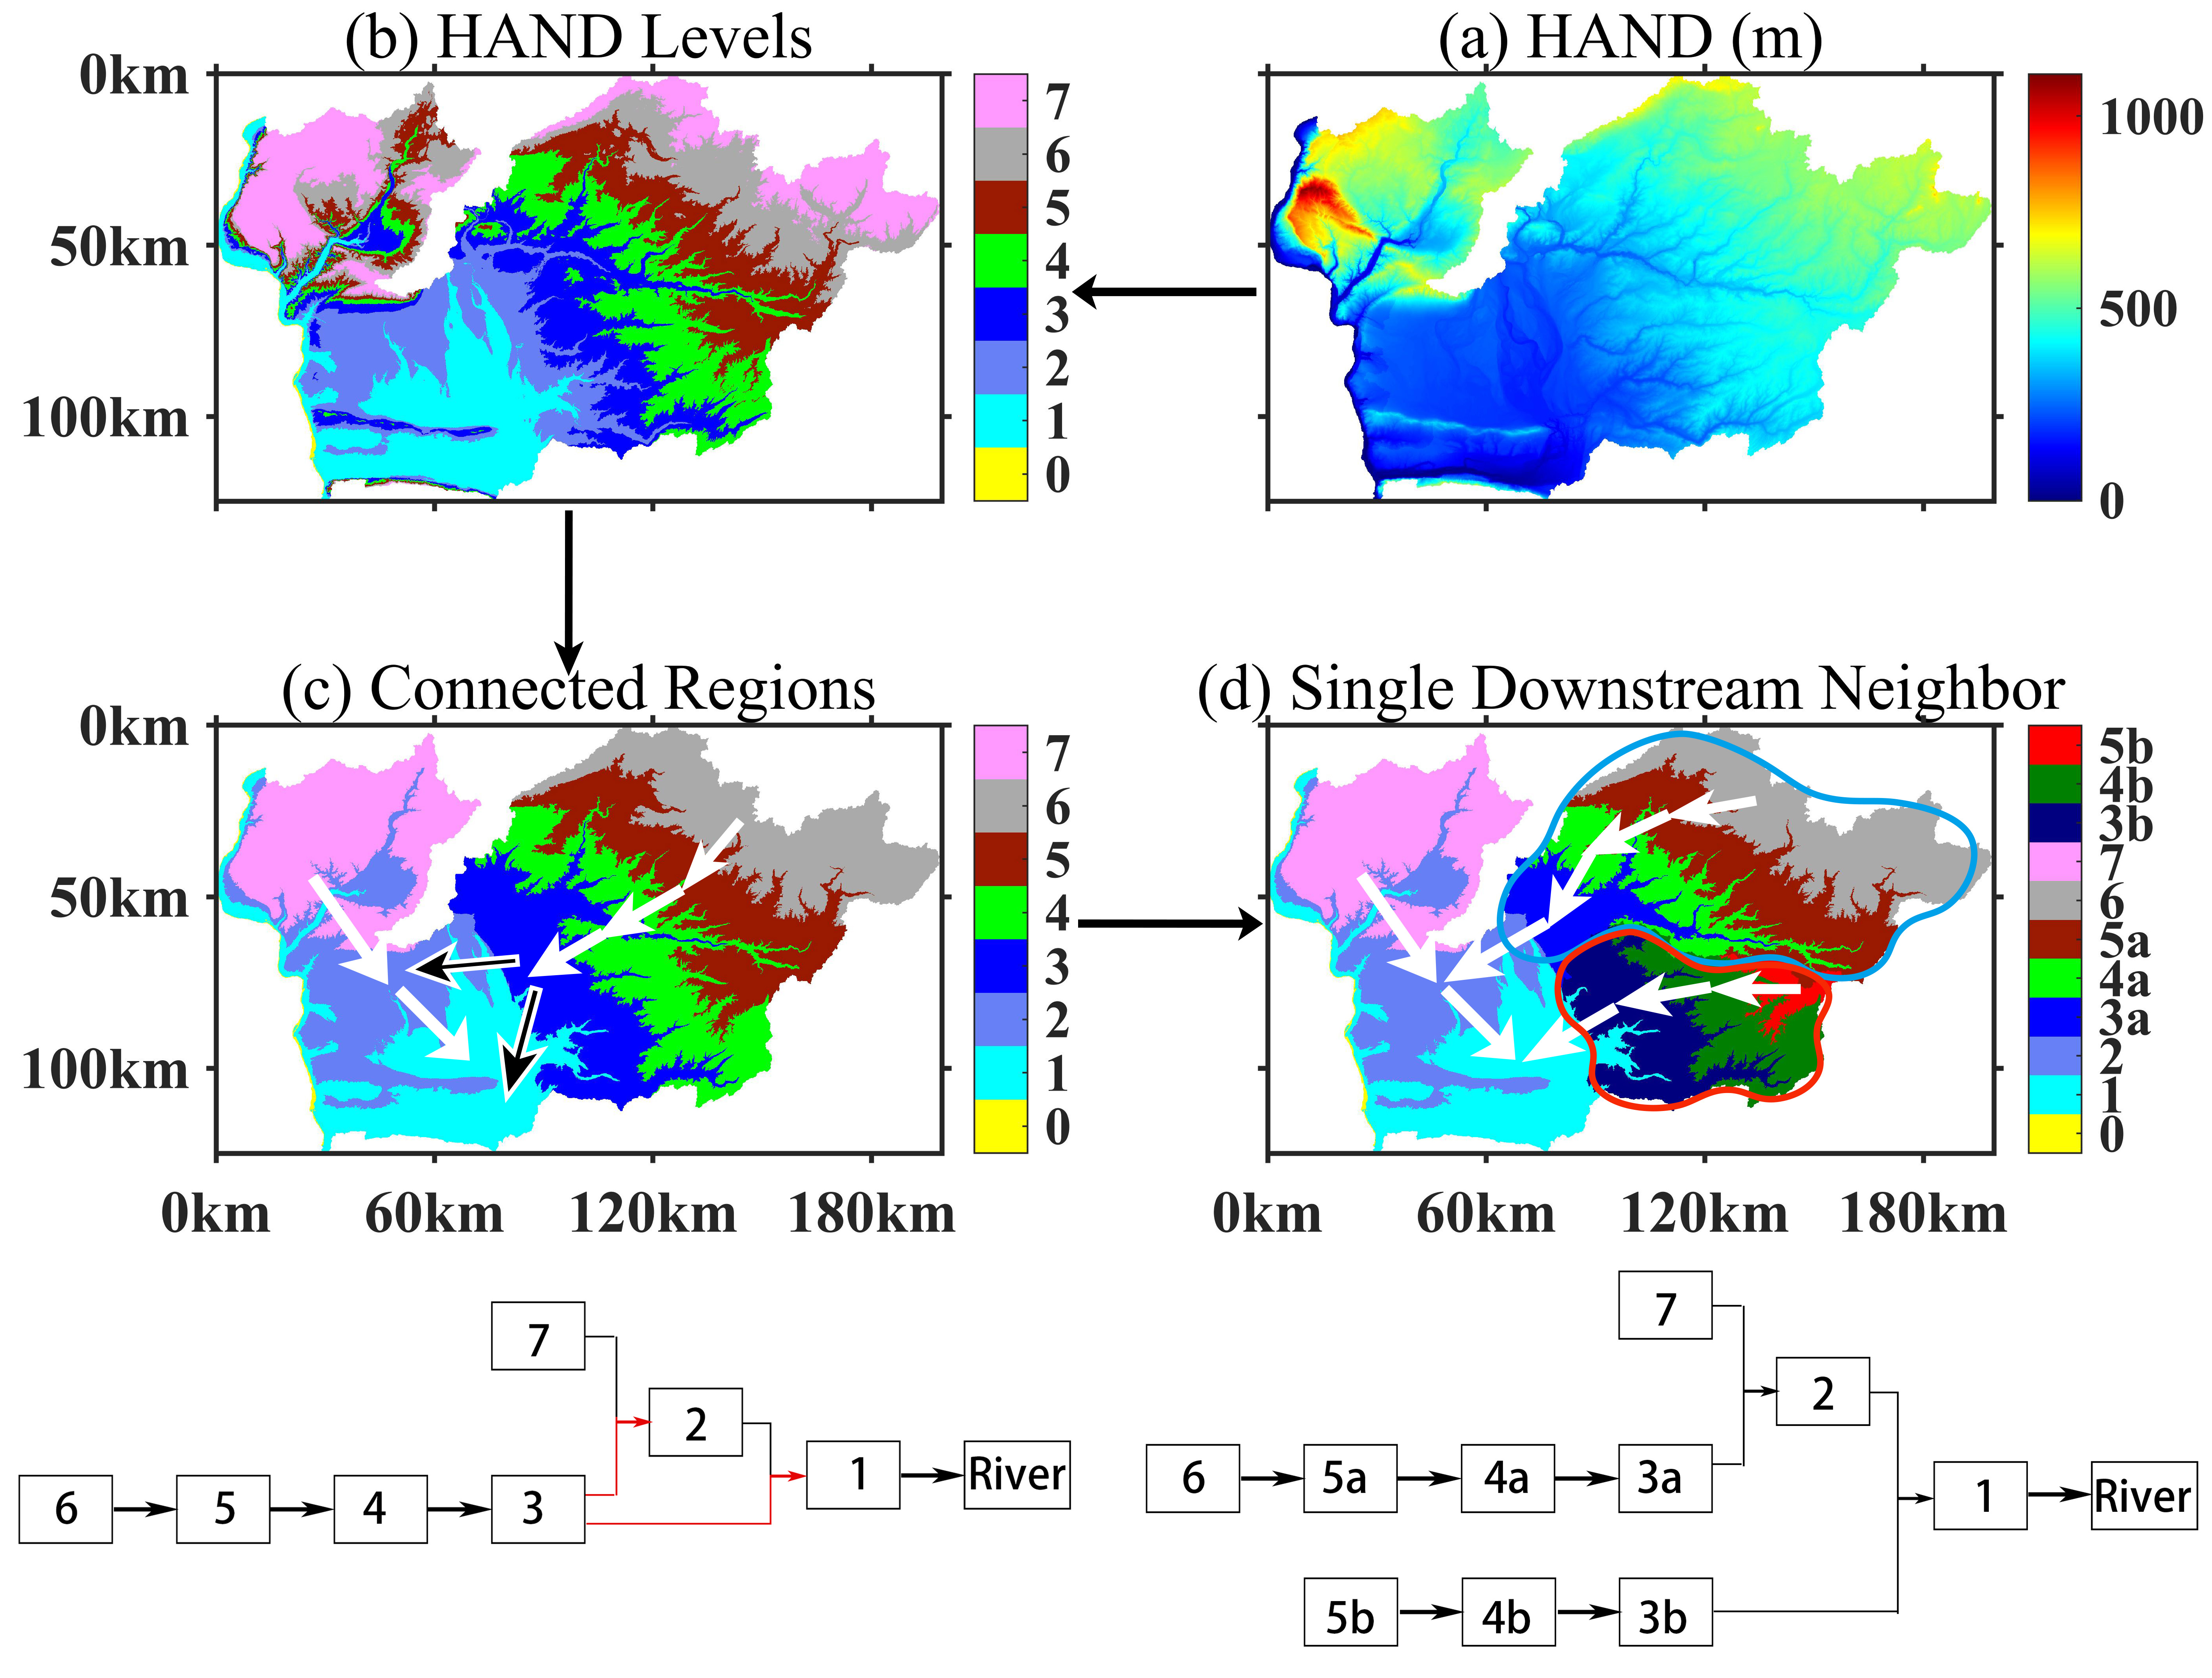
\includegraphics[width=\textwidth]{Figures/模式构架/高度带单元的约束示意图.jpg}
\caption[对高度带单元进行约束的作用]{对高度带单元进行约束的作用:a)排水高度(HAND);b)仅根据排水高度划分高度带单元;c)具有连通性的高度带单元;d)满足连通性和具有唯一下游单元的高度带单元。上图中的箭头表示水流的方向}
\label{fig:高度带单元约束示意}
\end{figure}
}

在流域单元网格中,每个流域单元关联了一段河道。目前未考虑河道向下游分叉的情况,因此,除入海口和内陆洼地单元外,每个流域单元都有唯一的下游单元,整个模拟区域的流域单元在水文上都是连通的(见图~\ref{fig:湖泊划分}~左)。

自然连通的湖泊设置为独立的单元,不受面积阈值的限制。生成流域单元网格时,首先使用HydroLAKES数据\citep{messager2016nc}将区域内的湖泊标识出来,再将模拟区域内的其余部分划分为流域单元。为了避免单个湖泊的面积过大,使用CVT算法\citep{du1999siam}对湖泊进行了进一步的划分(见图~\ref{fig:湖泊划分}~右)。
{
\begin{figure}[htbp]
\centering
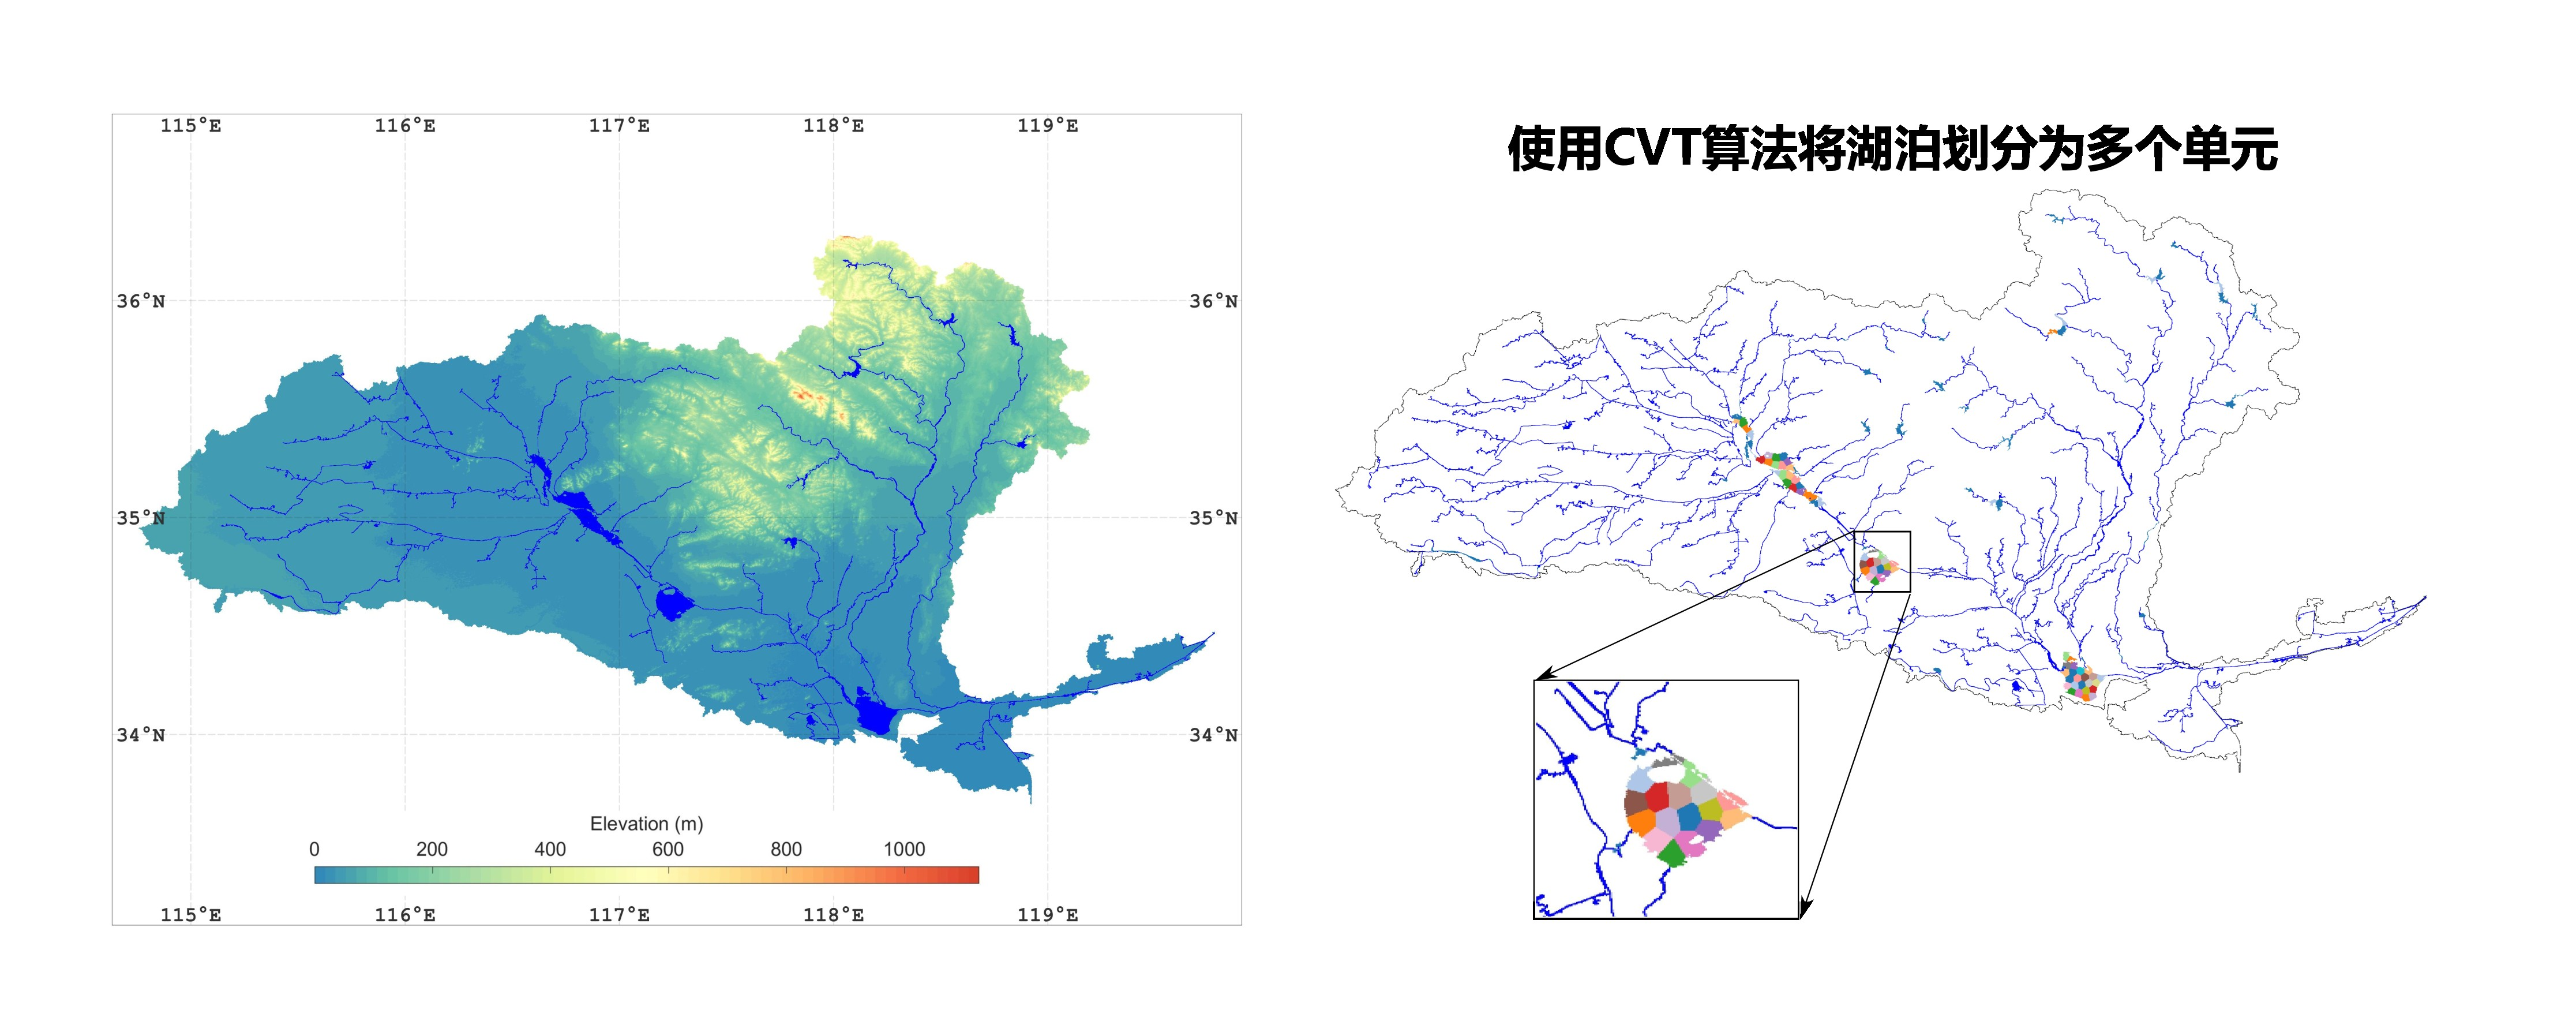
\includegraphics[width=\textwidth]{Figures/模式构架/湖泊划分.jpg}
\caption[流域单元网格中的湖泊]{流域单元网格中的湖泊。左图为模拟区域(淮河流域)的范围、高程以及河道和湖泊网络。右图表示采用CVT算法将湖泊区域进一步划分为更小的单元}
\label{fig:湖泊划分}
\end{figure}
}



\section{次网格结构}\label{次网格}
\begin{mymdframed}{代码}
本节对应的次网格类型可在\texttt{/include/define.h}中进行选择。
\end{mymdframed}
\subsection{次网格结构概述}
考虑到地表下垫面覆盖的异质性,CoLM对模式网格单元进一步划分次网格。
次网格是CoLM计算模拟的基本结构单元,通常称为patch(斑块)。
Patch是通过使用高分辨率的精细化网格数据,根据网格单元内部地表覆盖类型、植被功能类型、叶面积指数、土壤属性和地形等分布特征,按一定方式进行划分并聚合而来。Patch是用于模拟网格单元内部不同下垫面覆盖过程(对地表异质性考虑),同时也起到了减少计算量作用。


由patch可以组成按经纬度网格、流域单元网格(章节~\ref{流域单元网格})及非结构(章节~\ref{非结构网格})网格。
在patch尺度计算得到的通量按其所在网格覆盖比例进行面积加权平均,作为地表网格通量模拟结果。
地表状态或预报变量一般情况下亦是如此,在patch尺度计算得到的结果按照面积加权平均后作为模式结果输出。

{
\begin{figure}[htbp]
\centering
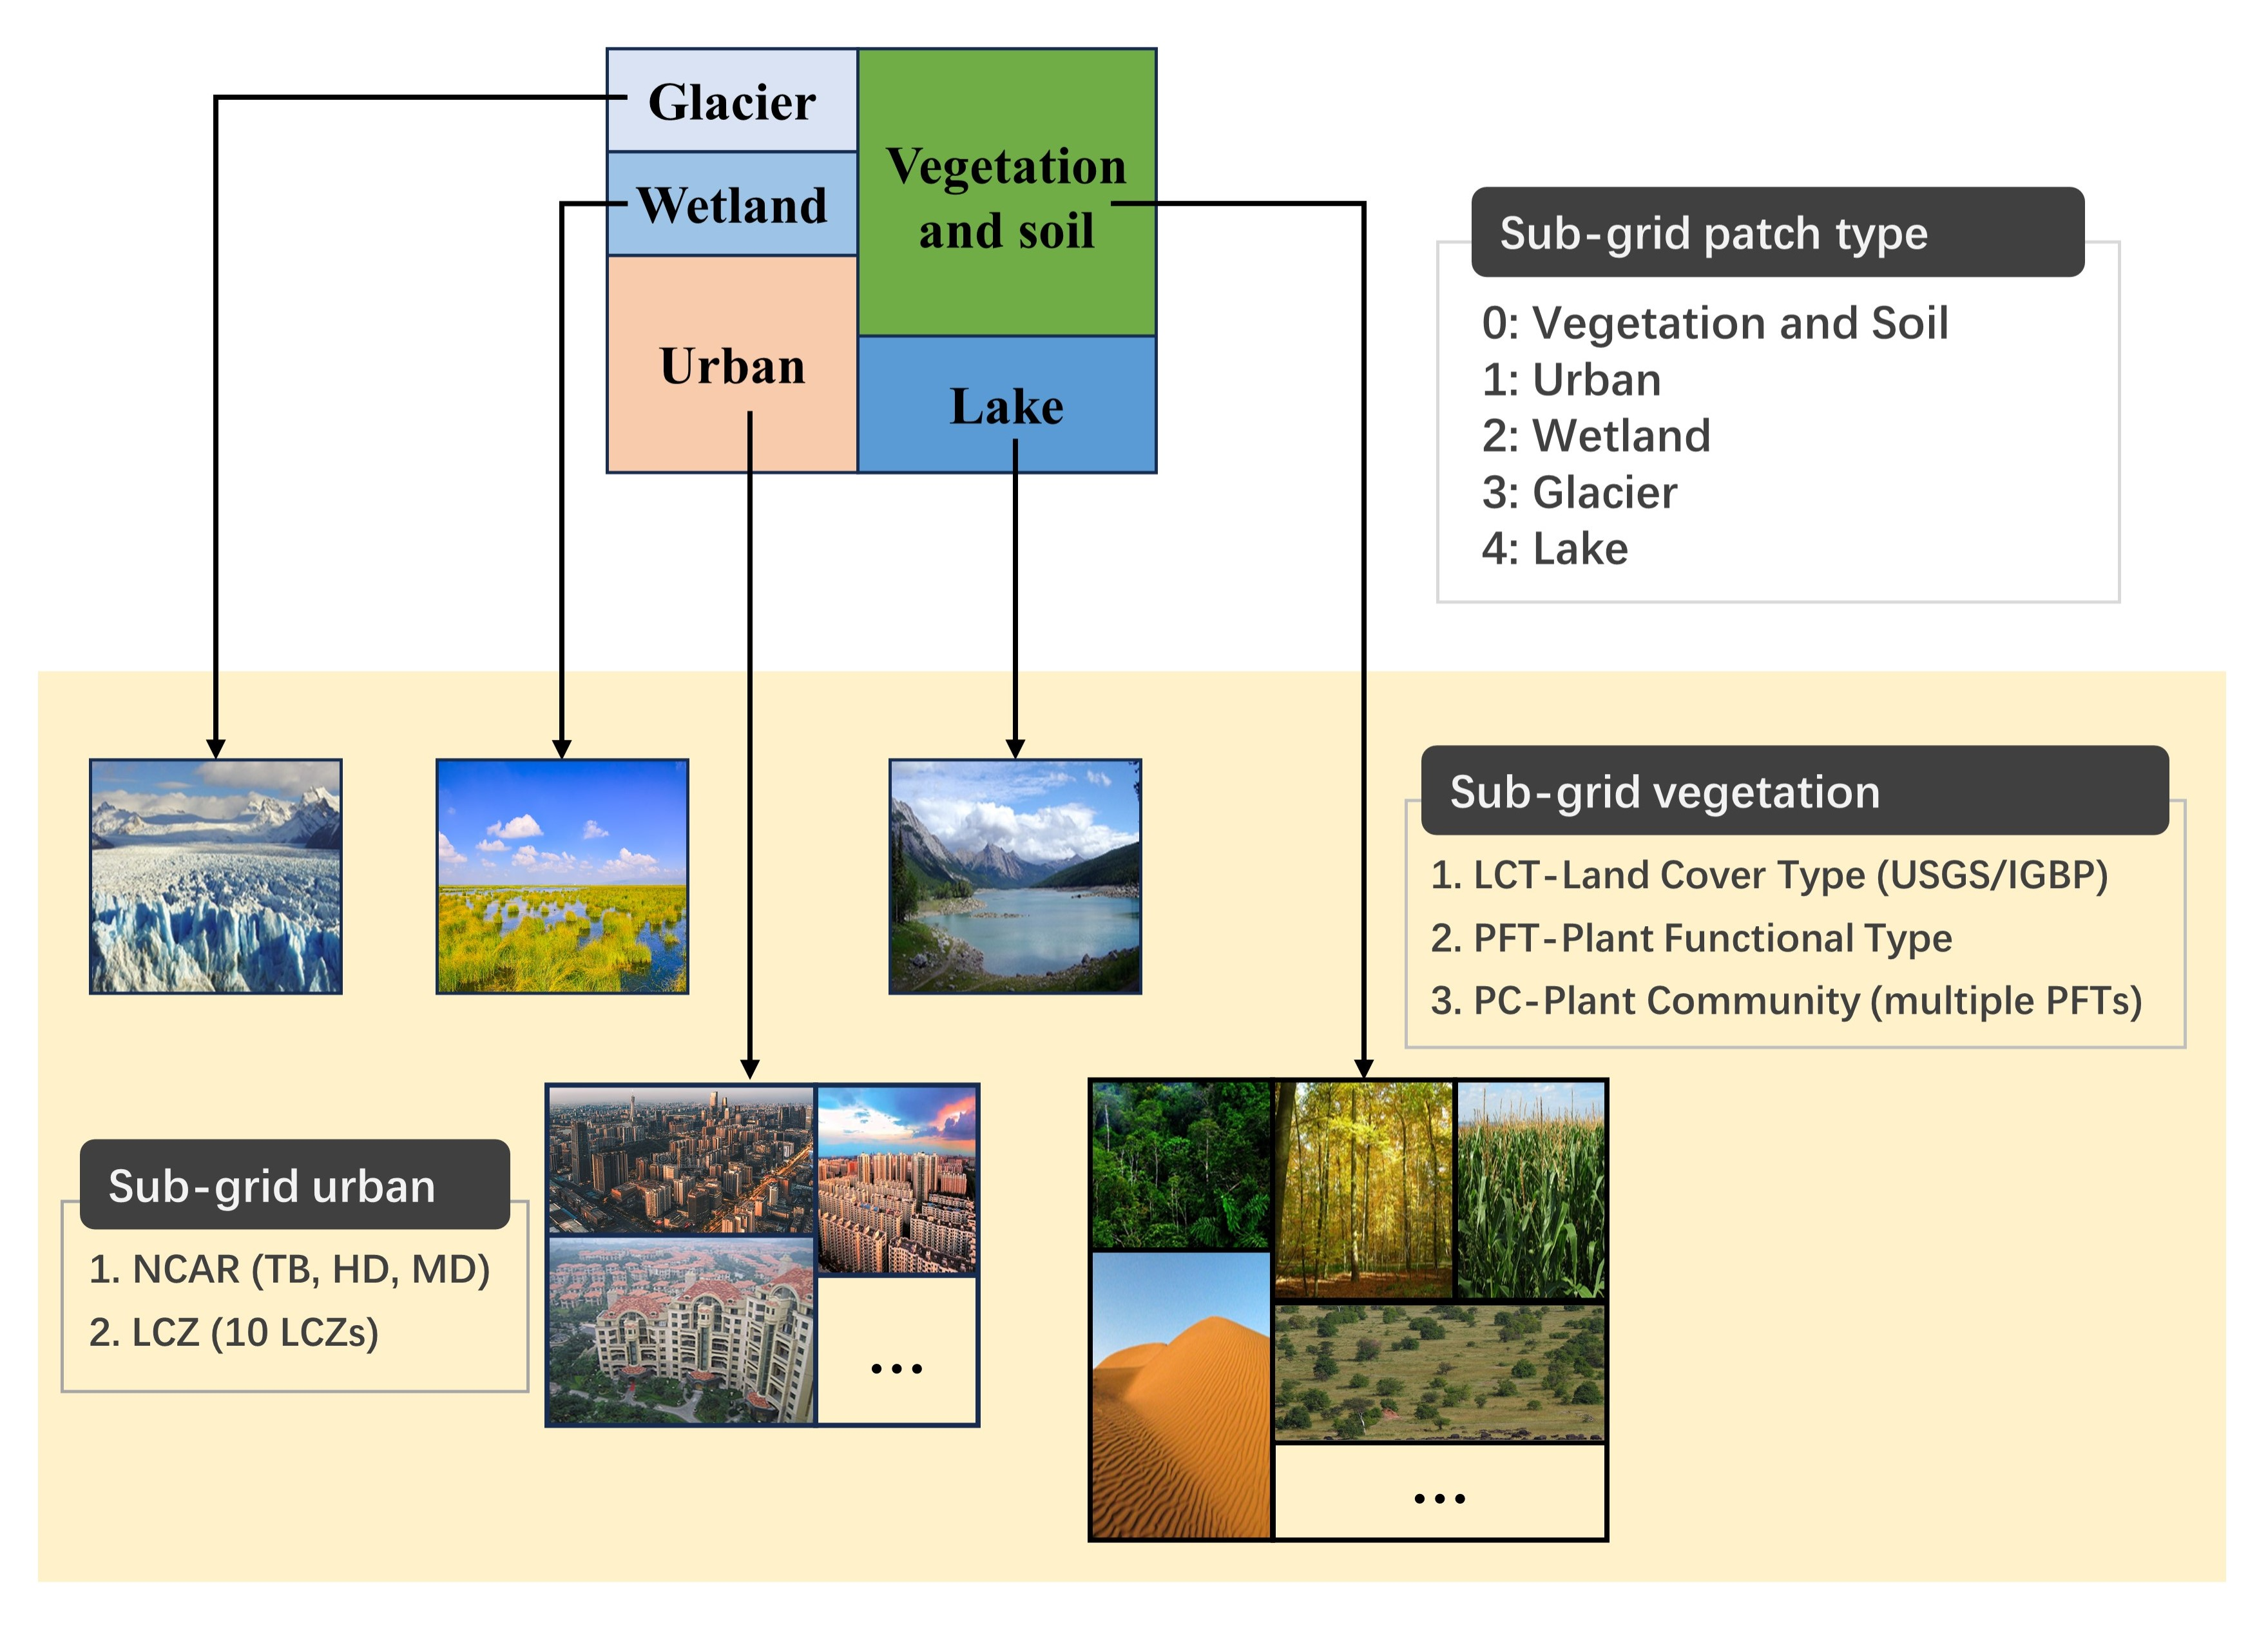
\includegraphics[width=\textwidth]{Figures/模式构架/CoLM次网格结构示意图-v2.jpg}
\caption[CoLM次网格结构示意图]{CoLM次网格结构示意图。次网格植被(Sub-grid vegetation)结构提供三种可选方式:LCT, PFT以及PC;当作物模式打开时,每种作物当成一种独立的PFT (CFT)进行模拟;当城市模式打开时,次网格城市(Sub-grid urban)结构提供两种可选方式:NCAR 3种城市分类和LCZ 10种分类}
\label{fig:次网格结构示意图}
\end{figure}
}


CoLM非海洋patch从大类上分为五类:植被(含裸土)、城市、湿地、冰川和水体,如图~\ref{fig:次网格结构示意图} 所示。在模式中的编号依次为0--4。其中植被和城市patch可根据不同类型进一步细分。

\subsection{植被次网格结构}\label{sec:植被次网格}
植被patch可以分为自然植被和作物。自然植被patch采用三种次网格植被结构进行表征(图~\ref{fig:植被次网格方案}):1) 地表覆盖类型---LCT (Land Cover Type);2) 植被功能型---PFT (Plant Function Type)和3) 植物群落---PC (Plant Community)。以上三种方式,模式运行时只能选择其中一种。

{
\begin{figure}[htbp]
\centering
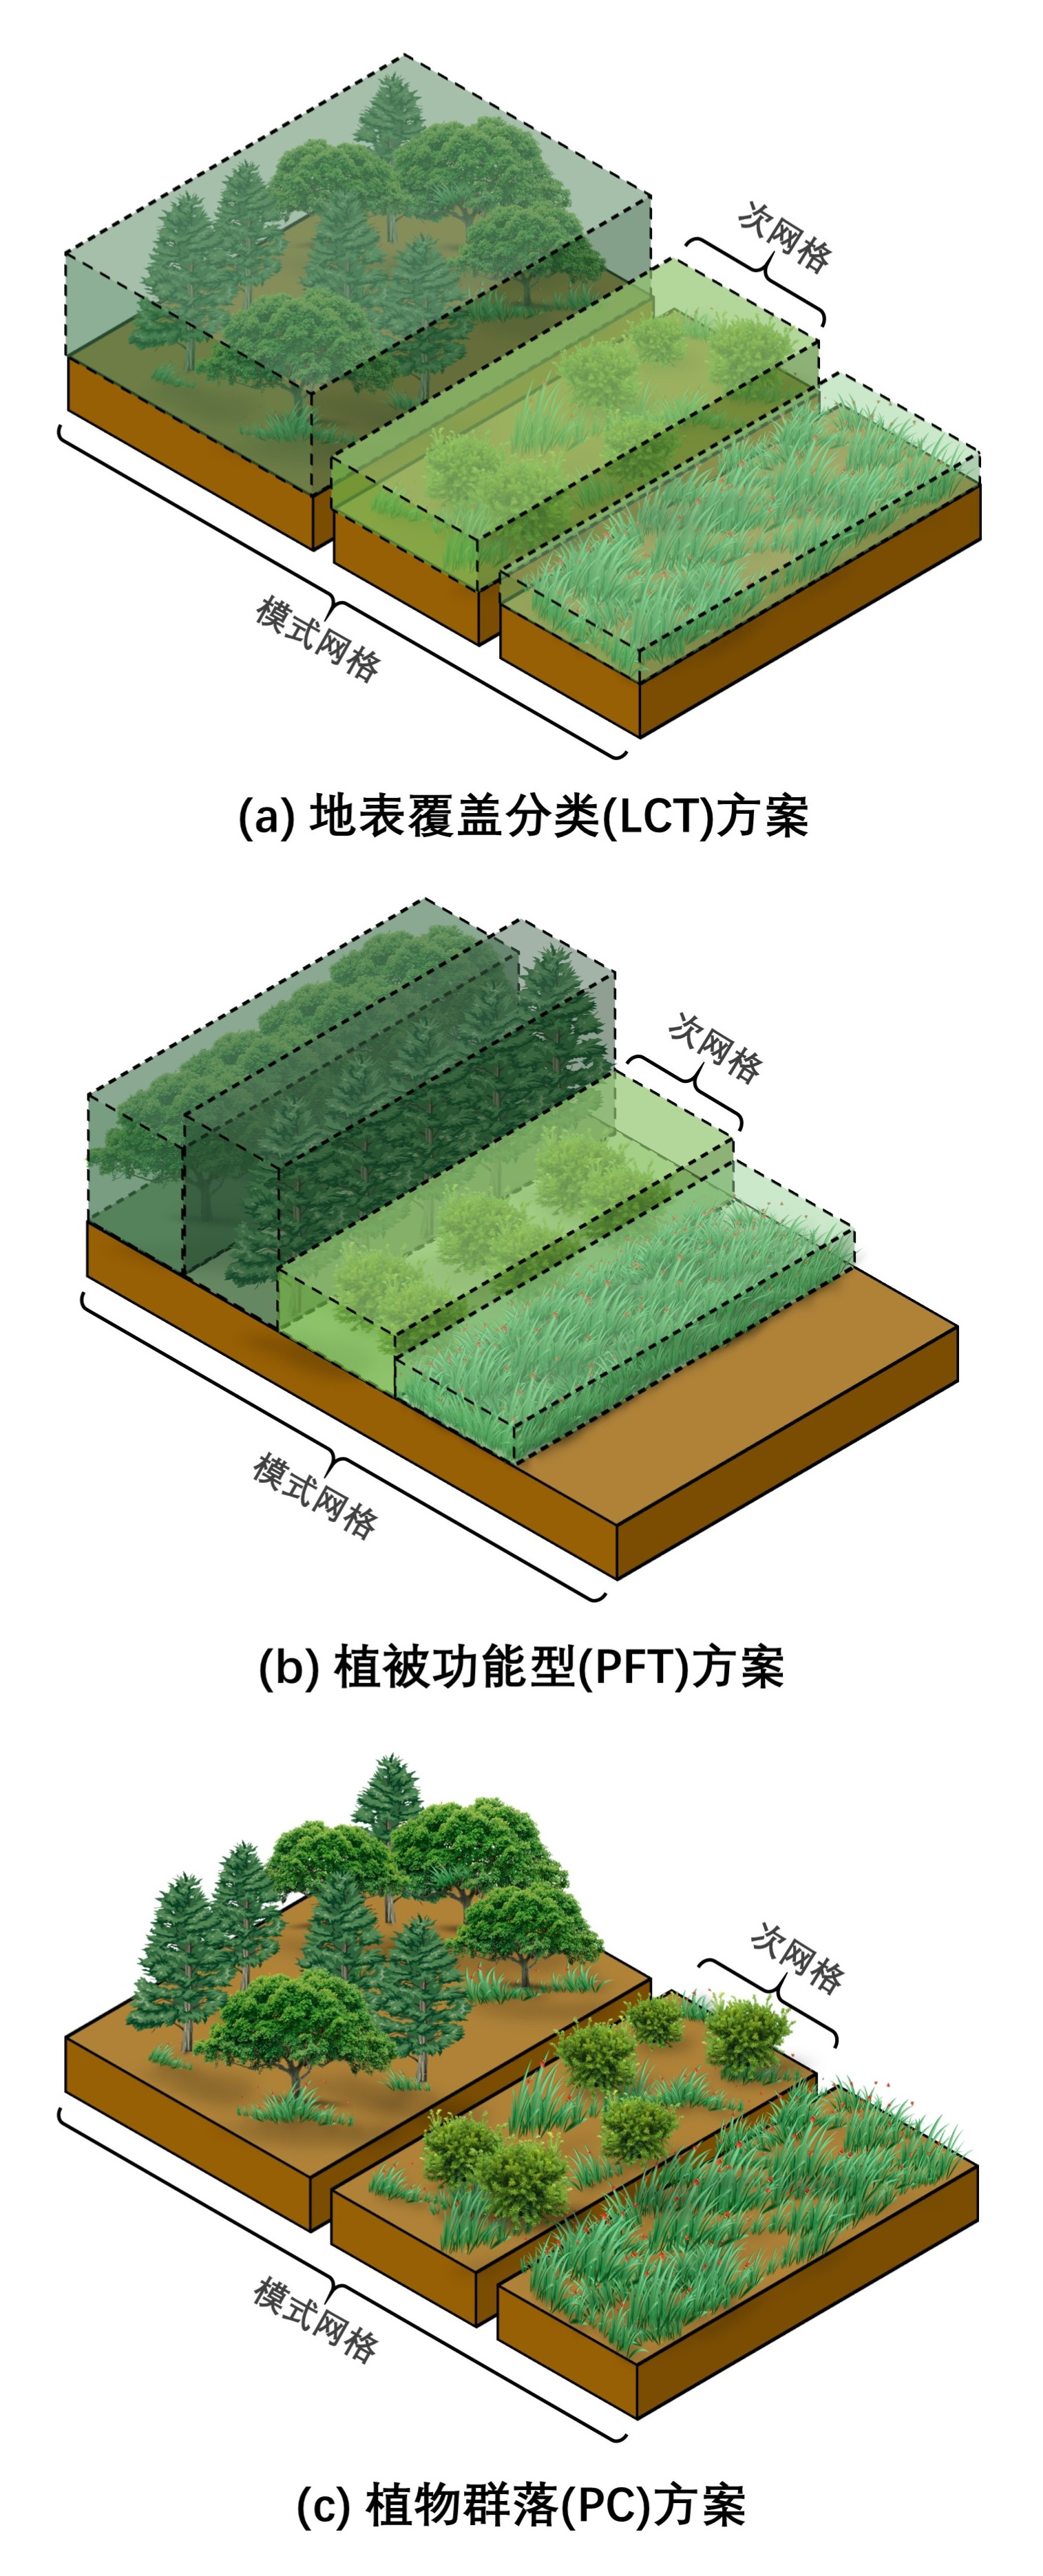
\includegraphics[width=0.55\textwidth]{Figures/模式构架/植被次网格方案示意图_v4.jpg}
\caption[CoLM植被次网格方案示意图]{CoLM植被次网格方案示意图。图中a (LCT方案)、b (PFT方案)中虚线框蒙版表示其包含的植被结构水平均一;图c (PC方案)与图a的差别在于缺少虚线框所示蒙版,即对次网格中的植被结构进行显式表达}
\label{fig:植被次网格方案}
\end{figure}
}

LCT方案为CoLM2014版原有方案(图~\ref{fig:植被次网格方案}a所示),即将某一地表覆盖类型可能包含的多种功能型植被当成混合(水平均一)植被进行模拟,其设置的相关参数可视为等效参数,图~\ref{fig:植被次网格方案}a中虚线框所示蒙版表示其中所包含植被结构水平均一。例如热带大草原,虽然可能包含树和草,但仍视为一种植被,因此相应的植被参数只有一套。

PFT是目前陆面模式(如CLM和JULES)常采用的次网格表征方式,也是本版本CoLM新添加的方式(图~\ref{fig:植被次网格方案}b所示)。
PFT方案是将每一个细网格地表覆盖类型进行拆解,得到其PFT的组成种类和各自面积占比,并将其聚合到模式网格中。同样,每种PFT植被结构也假设为水平均一,在图~\ref{fig:植被次网格方案}b中用虚线蒙版表示。本版本CoLM PFT方案类似于CLM PFT方案,即模式格点中的所有PFT作为1个植被patch,共享土壤水热等环境,但各PFT的辐射和通量等过程计算相对独立。

{
\begin{figure}[htbp]
\centering
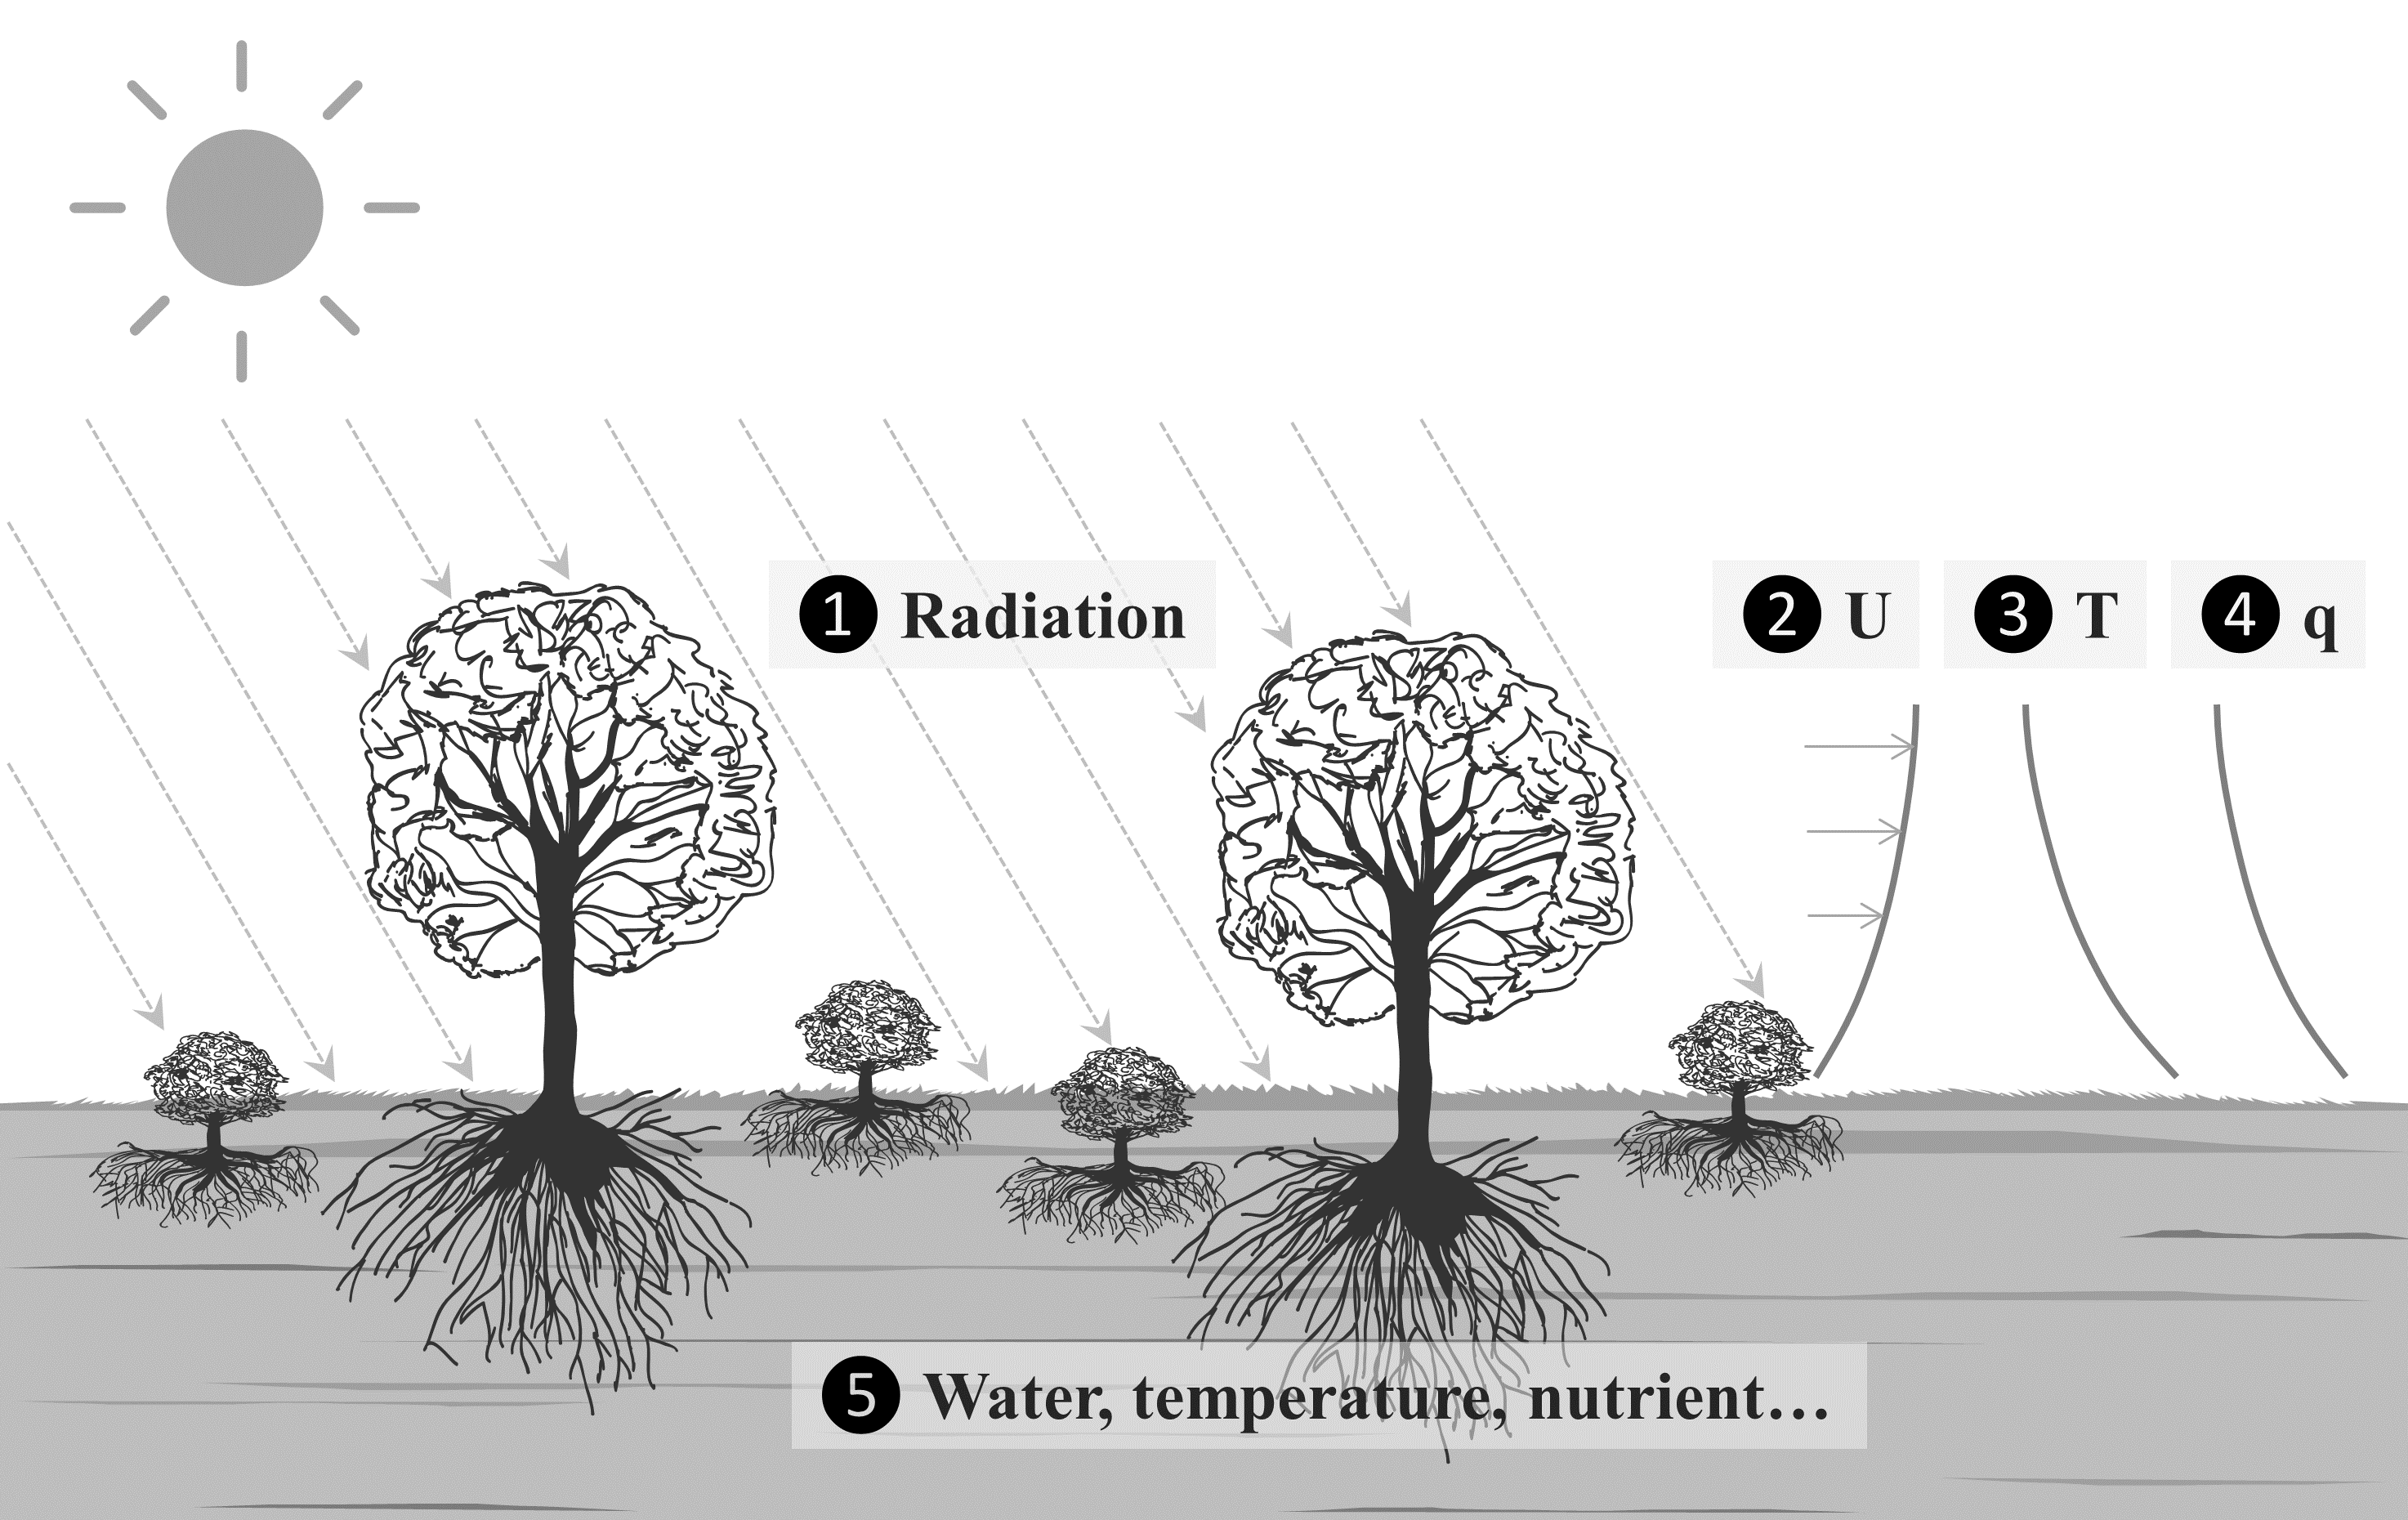
\includegraphics[width=0.95\textwidth]{Figures/模式构架/植物群落示意图.png}
\caption[CoLM植物群落(PC)次网格概念示意图]{CoLM植物群落(PC)次网格概念示意图。同一植物群落中的PFT环境共享,资源竞争,包括辐射、风速、水热及营养元素等}
\label{fig:植物群落示意图}
\end{figure}
}

PC方案保留LCT方案中模拟对象,即地表覆盖类型,同时还进一步对LCT中的地表覆盖植被类型进行PFT细分(图~\ref{fig:植被次网格方案}c所示)。
不同于LCT方案把某一类型地表覆盖的所有植被视为混合植被,PC方案对某一地表覆盖类型所组成的PFT进行显式表达计算,所有PFT在同一次网格patch中共享辐射、风、水热及营养元素等环境,同时辐射和通量计算等过程PFT之间相互影响、同时求解,即考虑了PFT之间的共存与竞争(如图~\ref{fig:植物群落示意图} 所示)。这一方案类似于植物群落的概念,故命名为PC (Plant Community)方案。

LCT方案所依赖的地表覆盖类型数据可以直接由USGS (章节~\ref{USGS地表覆盖数据})或者MODIS-IGBP地表覆盖数据获取(章节~\ref{IGBP地表覆盖数据})。PFT和PC方案所需要的植被结构及属性数据由MODIS-IGBP地表覆盖数据加以其他辅助数据制作而成(章节~\ref{PFTPC数据及其依赖数据})。

对于作物patch,当作物模式未打开时,作物被当成一种特殊的自然植被进行模拟;当打开作物模式时,每个模式格点根据包含的作物分类及组成比例(外部数据读取)分别建立相互独立的patch进行模拟计算,方式类似PFT方案,但不同之处在于每种作物的土壤计算保持独立,不共享土壤水热等环境。

\subsection{城市次网格结构}
\begin{mymdframed}{代码}
本节对应的城市次网格类型可在\texttt{MOD\_Namelist.F90}中进行选择。
\end{mymdframed}

城市patch与作物类似,当城市模式未打开时,城市被当成一种地表覆盖进行模拟,即薄板城市模型(Slab Urban);
当城市模式打开时,每个模式格点根据包含的城市类型和组成比例(根据几何参数)分别建立相互独立的patch进行模拟计算。

{
\begin{figure}[htbp]
\centering
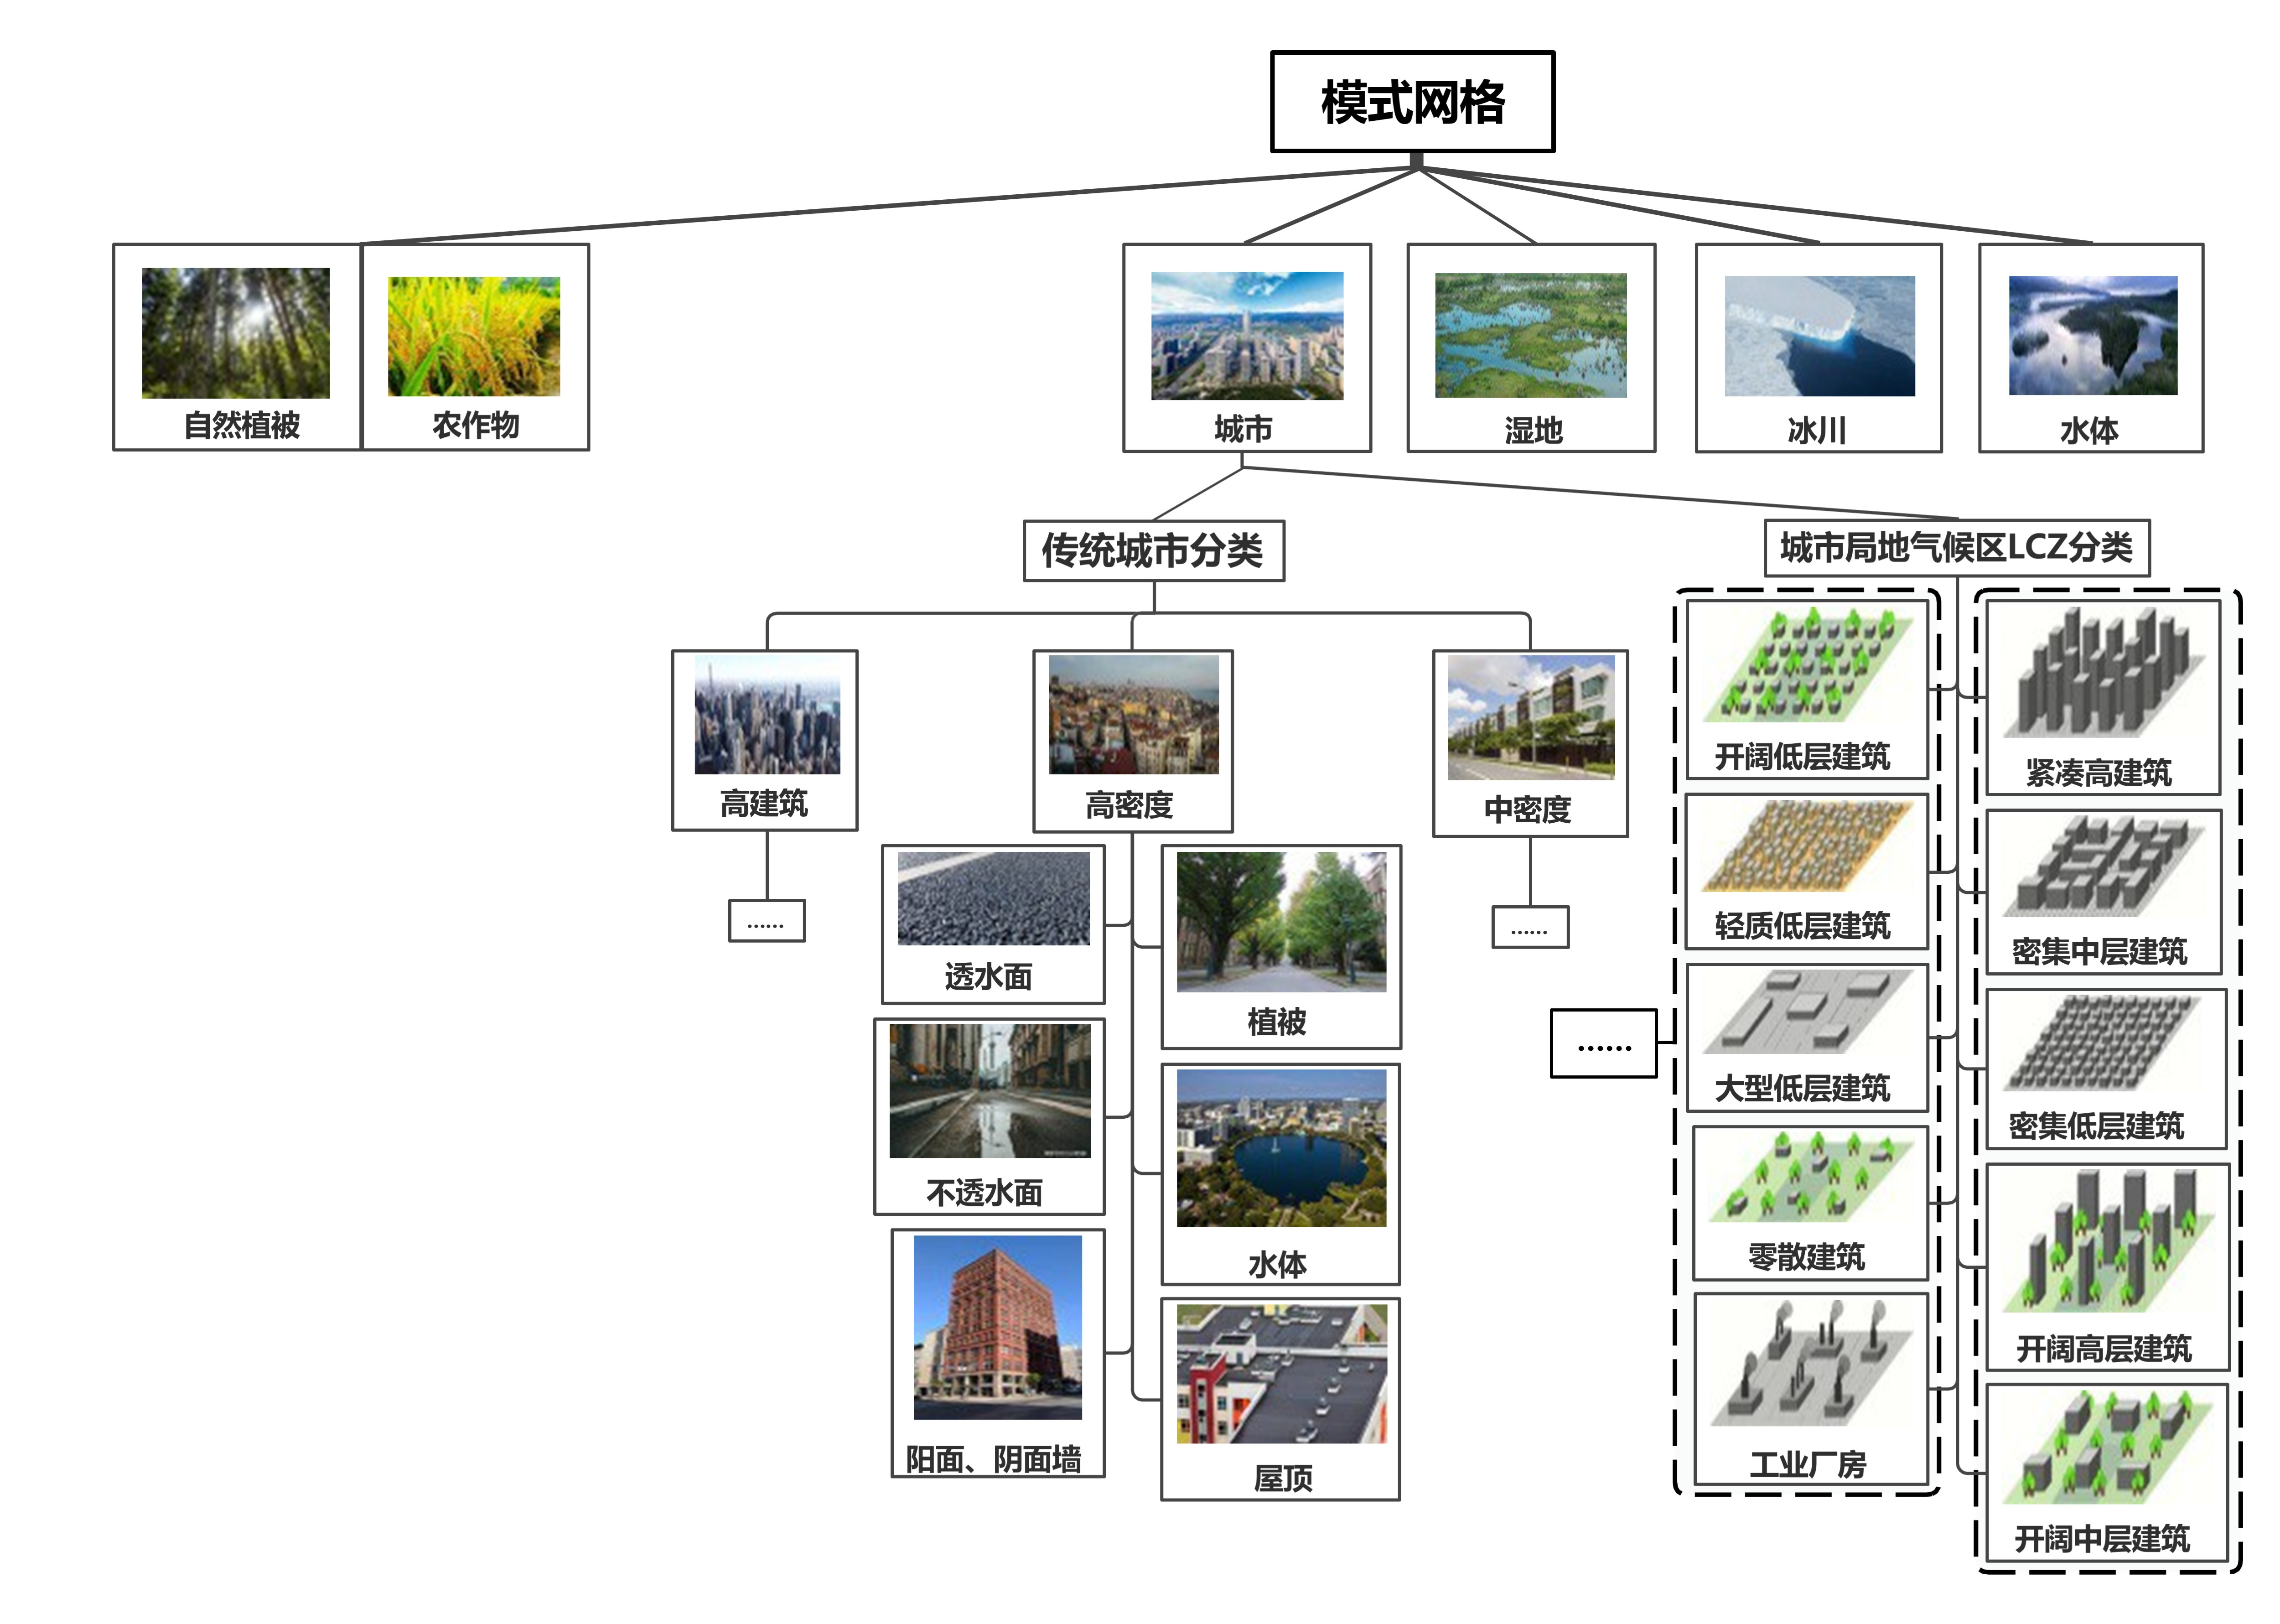
\includegraphics[width=0.95\textwidth]{Figures/模式构架/CoLM城市次网格示意图.jpg}
\caption[CoLM城市模式次网格结构示意图]{CoLM城市模式次网格结构示意图}
\label{fig:城市次网格}
\end{figure}
}

目前城市分类提供两种方式(图~\ref{fig:城市次网格}):
\begin{enumerate}
    \item 根据城市密度分为高建筑-TB、高密度-HD和中密度-MD 3类(基于NCAR CLMU城市模式);
    \item 根据城市局地气候区(LCZ,Local Climate Zone)分为10类。
\end{enumerate}
每种城市类型由屋顶、(地面)不透水面、透水面、阴/阳面墙、植被和水体组成。
城市分类及其相关属性数据主要从外部文件读取(章节~\ref{城市数据})。

\section{植被、土壤和积雪的垂直分层}\label{土壤和积雪的垂直分层}

{
\begin{figure}[htbp]
\centering
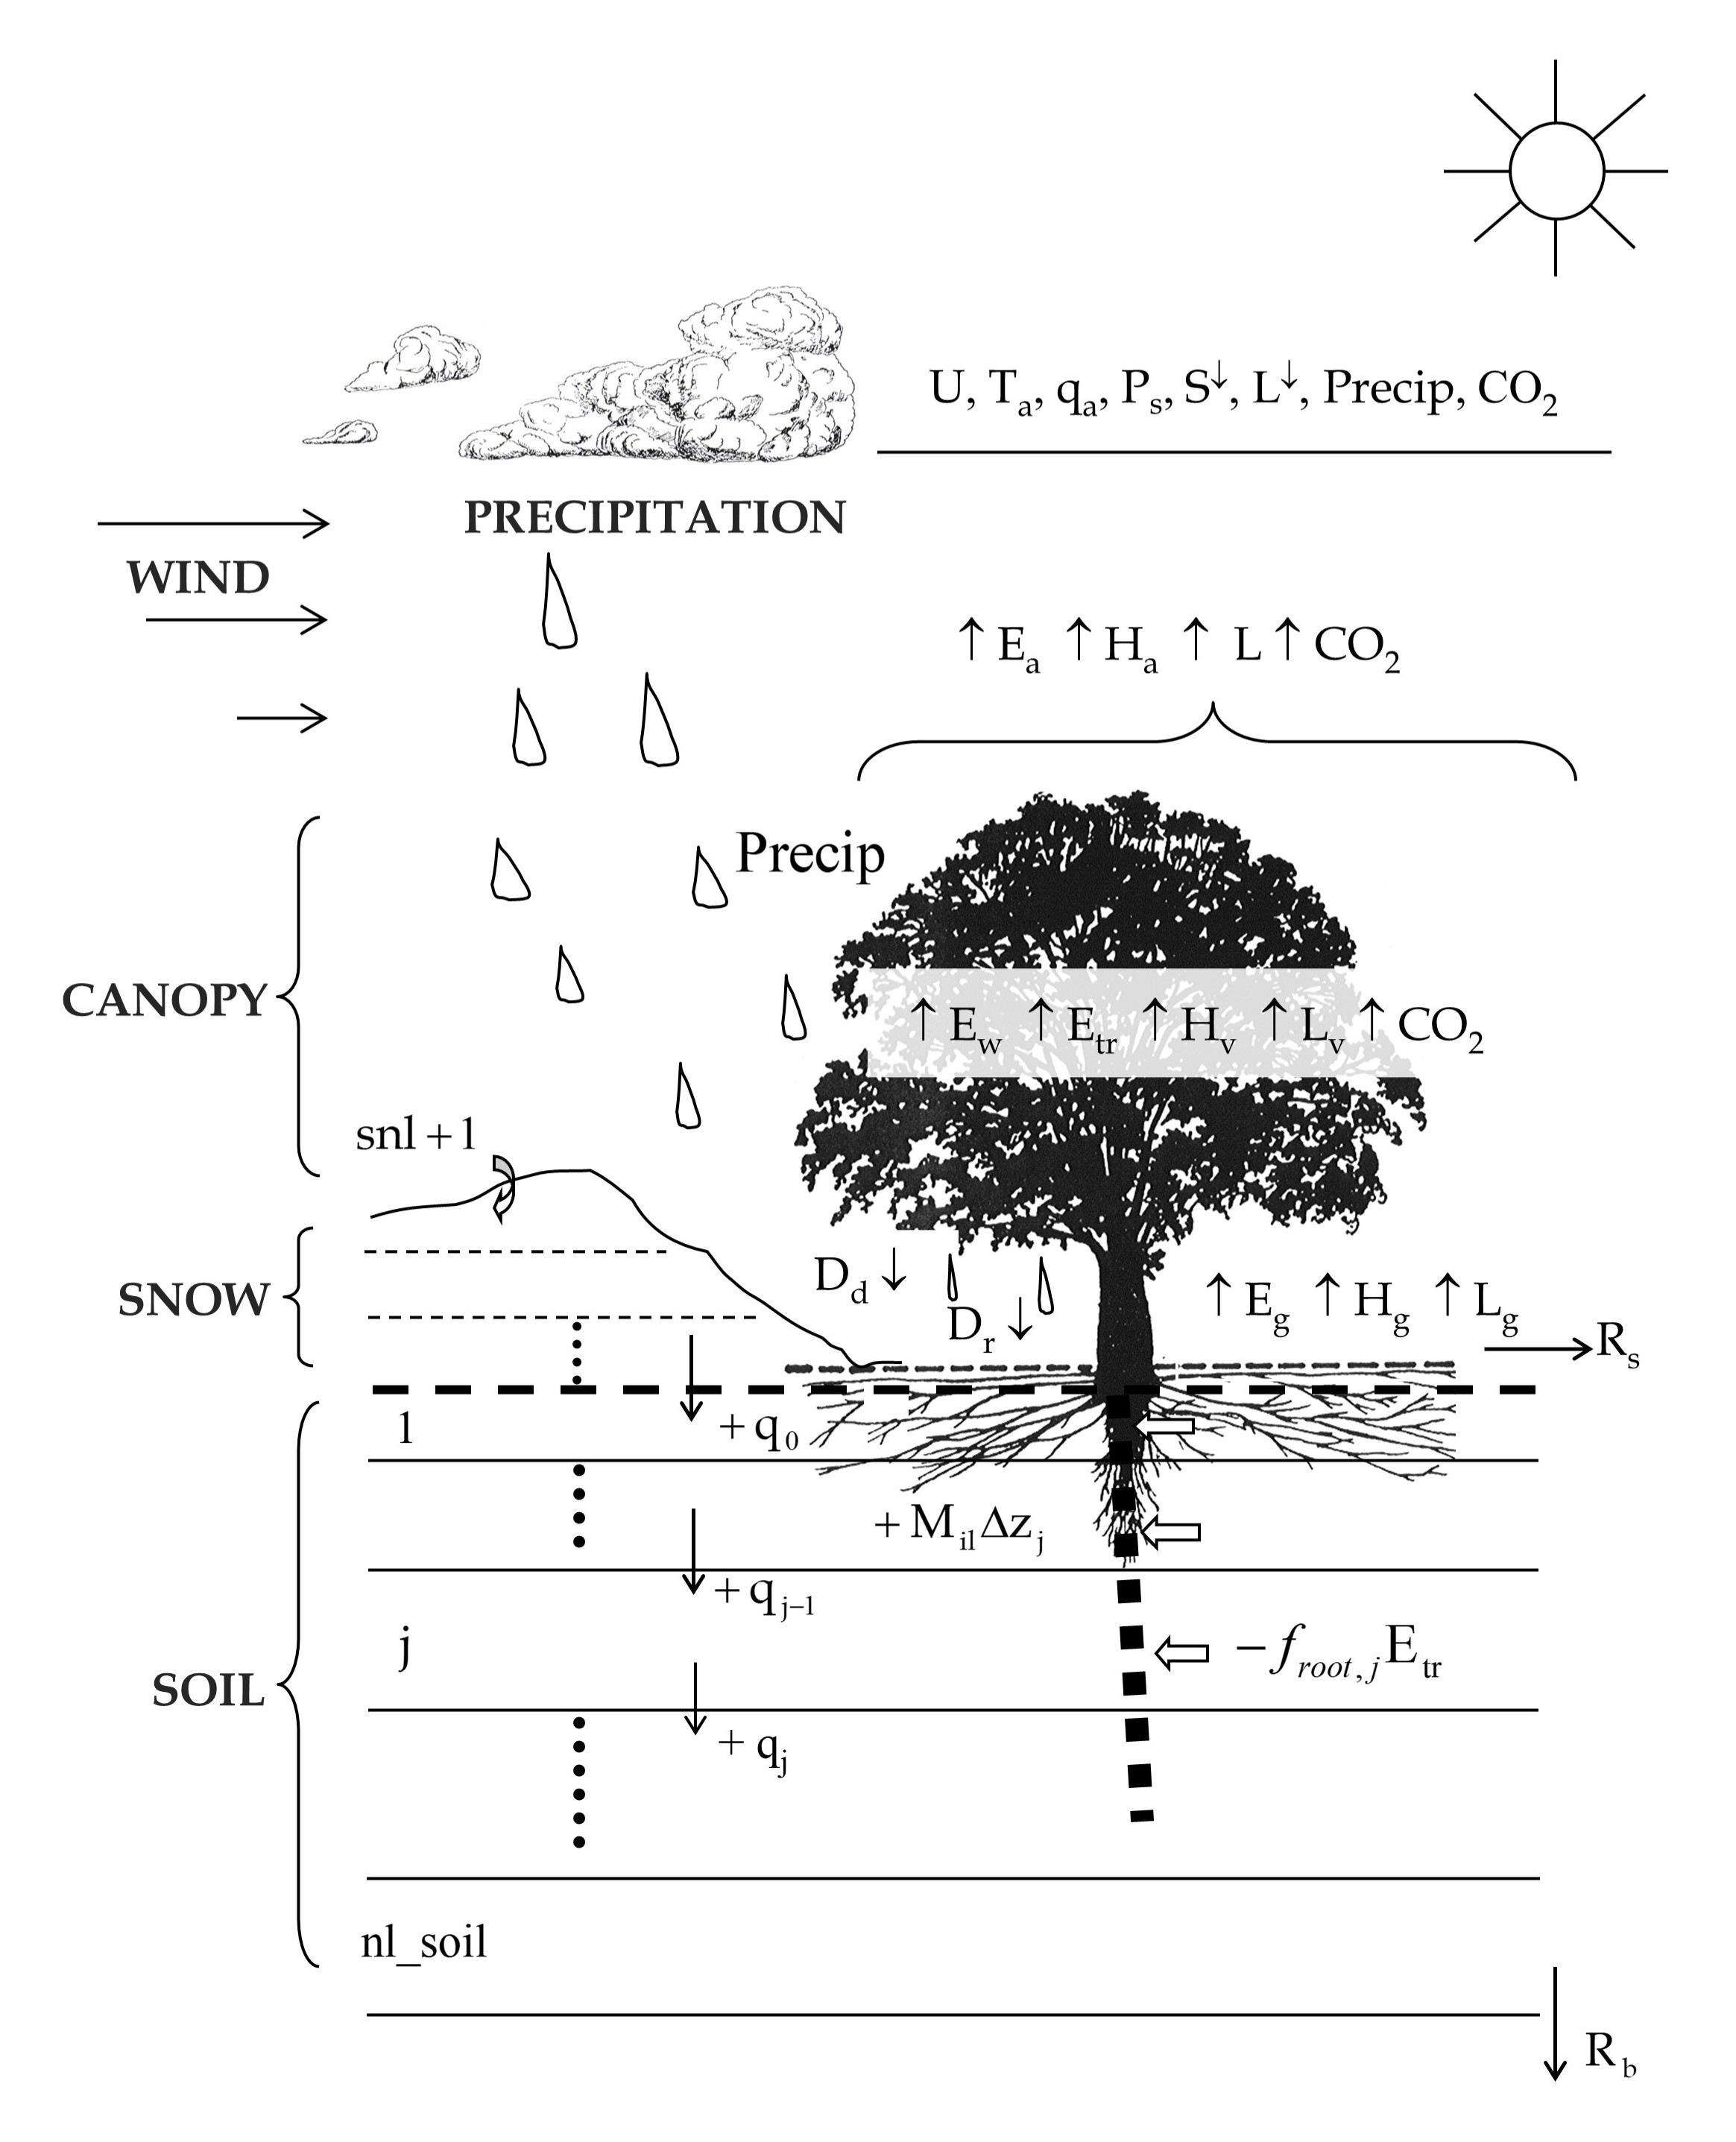
\includegraphics[width=0.9\textwidth]{Figures/模式构架/CoLM模式概念图.jpg}
\caption[CoLM植被、土壤和积雪垂直分层示意图]{CoLM植被、土壤和积雪垂直分层示意图}
\label{fig:CoLM垂直分层}
\end{figure}
}

CoLM植被、土壤和积雪的垂直分层如图~\ref{fig:CoLM垂直分层} 所示。

CoLM可根据次网格类型(章节~\ref{sec:植被次网格})将植被按照单层或最多三层进行模拟。对于单层植被(LCT和PFT植被次网格),采用双大叶模型进行模拟\citep{dai2004two};对于多层植被(PC植被次网格),每层植被的各PFT采用三维植被模型(章节~\ref{三维植被辐射传输模型} 和~\ref{三维植被湍流}),并结合双大叶模型进行模拟。

CoLM默认将土壤分为10层,每一层土壤的中心深度$z_i$~(m)定义为:
\begin{equation}
z_{i} = f_{s}\left\{ \exp{\left\lbrack 0.5(i - 0.5) \right\rbrack} - 1 \right\}
\end{equation}
其中尺度因子$f_s=0.025$. 因为土壤水热梯度在接近土壤与大气的交界面时往往较大,采用指数定义可以保证土壤接近表面时得到更细的分层。每一层土壤的厚度$\Delta z_i$~(m)计算为:
\begin{equation}
\Delta z_{i}=\left\{\begin{array}{ll}0.5\left(z_{1}+z_{2}\right) & i=1 \\
0.5\left(z_{i+1}-z_{i-1}\right) & i=2, \ldots, 9 \\ 
z_{10}-z_{9} & i=10\end{array}\right.
\end{equation}
相邻两层土壤交界处的深度$z_{h,i}$ (m)可计算为:
\begin{equation}
z_{h, i}=\left\{\begin{array}{ll}0.5\left(z_{i}+z_{i+1}\right) & i=1, \ldots, 9 \\
z_{10}+0.5 \Delta z_{10} & i=10\end{array}\right.
\end{equation}
CoLM中每层土壤中心的深度及每层下边界的深度见表~\ref{table:土壤分层}。

\begin{table}[b]
\caption{CoLM中的土壤分层(单位:米)} \label{table:土壤分层}
\centering \renewcommand{\arraystretch}{1.2} \footnotesize
\begin{tabular}{ccccccccccc}
\toprule
层 & 1 & 2 & 3 & 4 & 5 & 6 & 7 & 8 & 9 & 10 \\
\midrule
中心位置 & 0.0071 & 0.0279 & 0.0623 & 0.1189 & 0.2122 & 0.3661 & 0.6198 & 1.0380 & 1.7276 & 2.8646 \\
下边界位置 & 0.0175 & 0.0451 & 0.0906 & 0.1655 & 0.2891 & 0.4929 & 0.8289 & 1.3828 & 2.2961 & 3.4331 \\
\bottomrule
\end{tabular} 
\end{table}


雪盖位于土壤之上,可根据其厚度划分为至多5层。为与土壤层编号一致,
这里与土壤表层相邻的雪层记为第0层,逐渐向上依次记为第 -1 层直至至多为第 -4 层。
记$snl$为划分的雪层总层数的相反数,则最上层雪层即为第$snl+1$层。记雪层的厚度为$z_{sno}$,当$z_{sno}<0.01$时,这时积雪较少,不单独划分为层,$snl=0$,当$z_{sno}\geqslant 0.01$时,积雪分层的方案见图~\ref{fig:积雪分层}。

{
\begin{figure}[htbp]
\centering
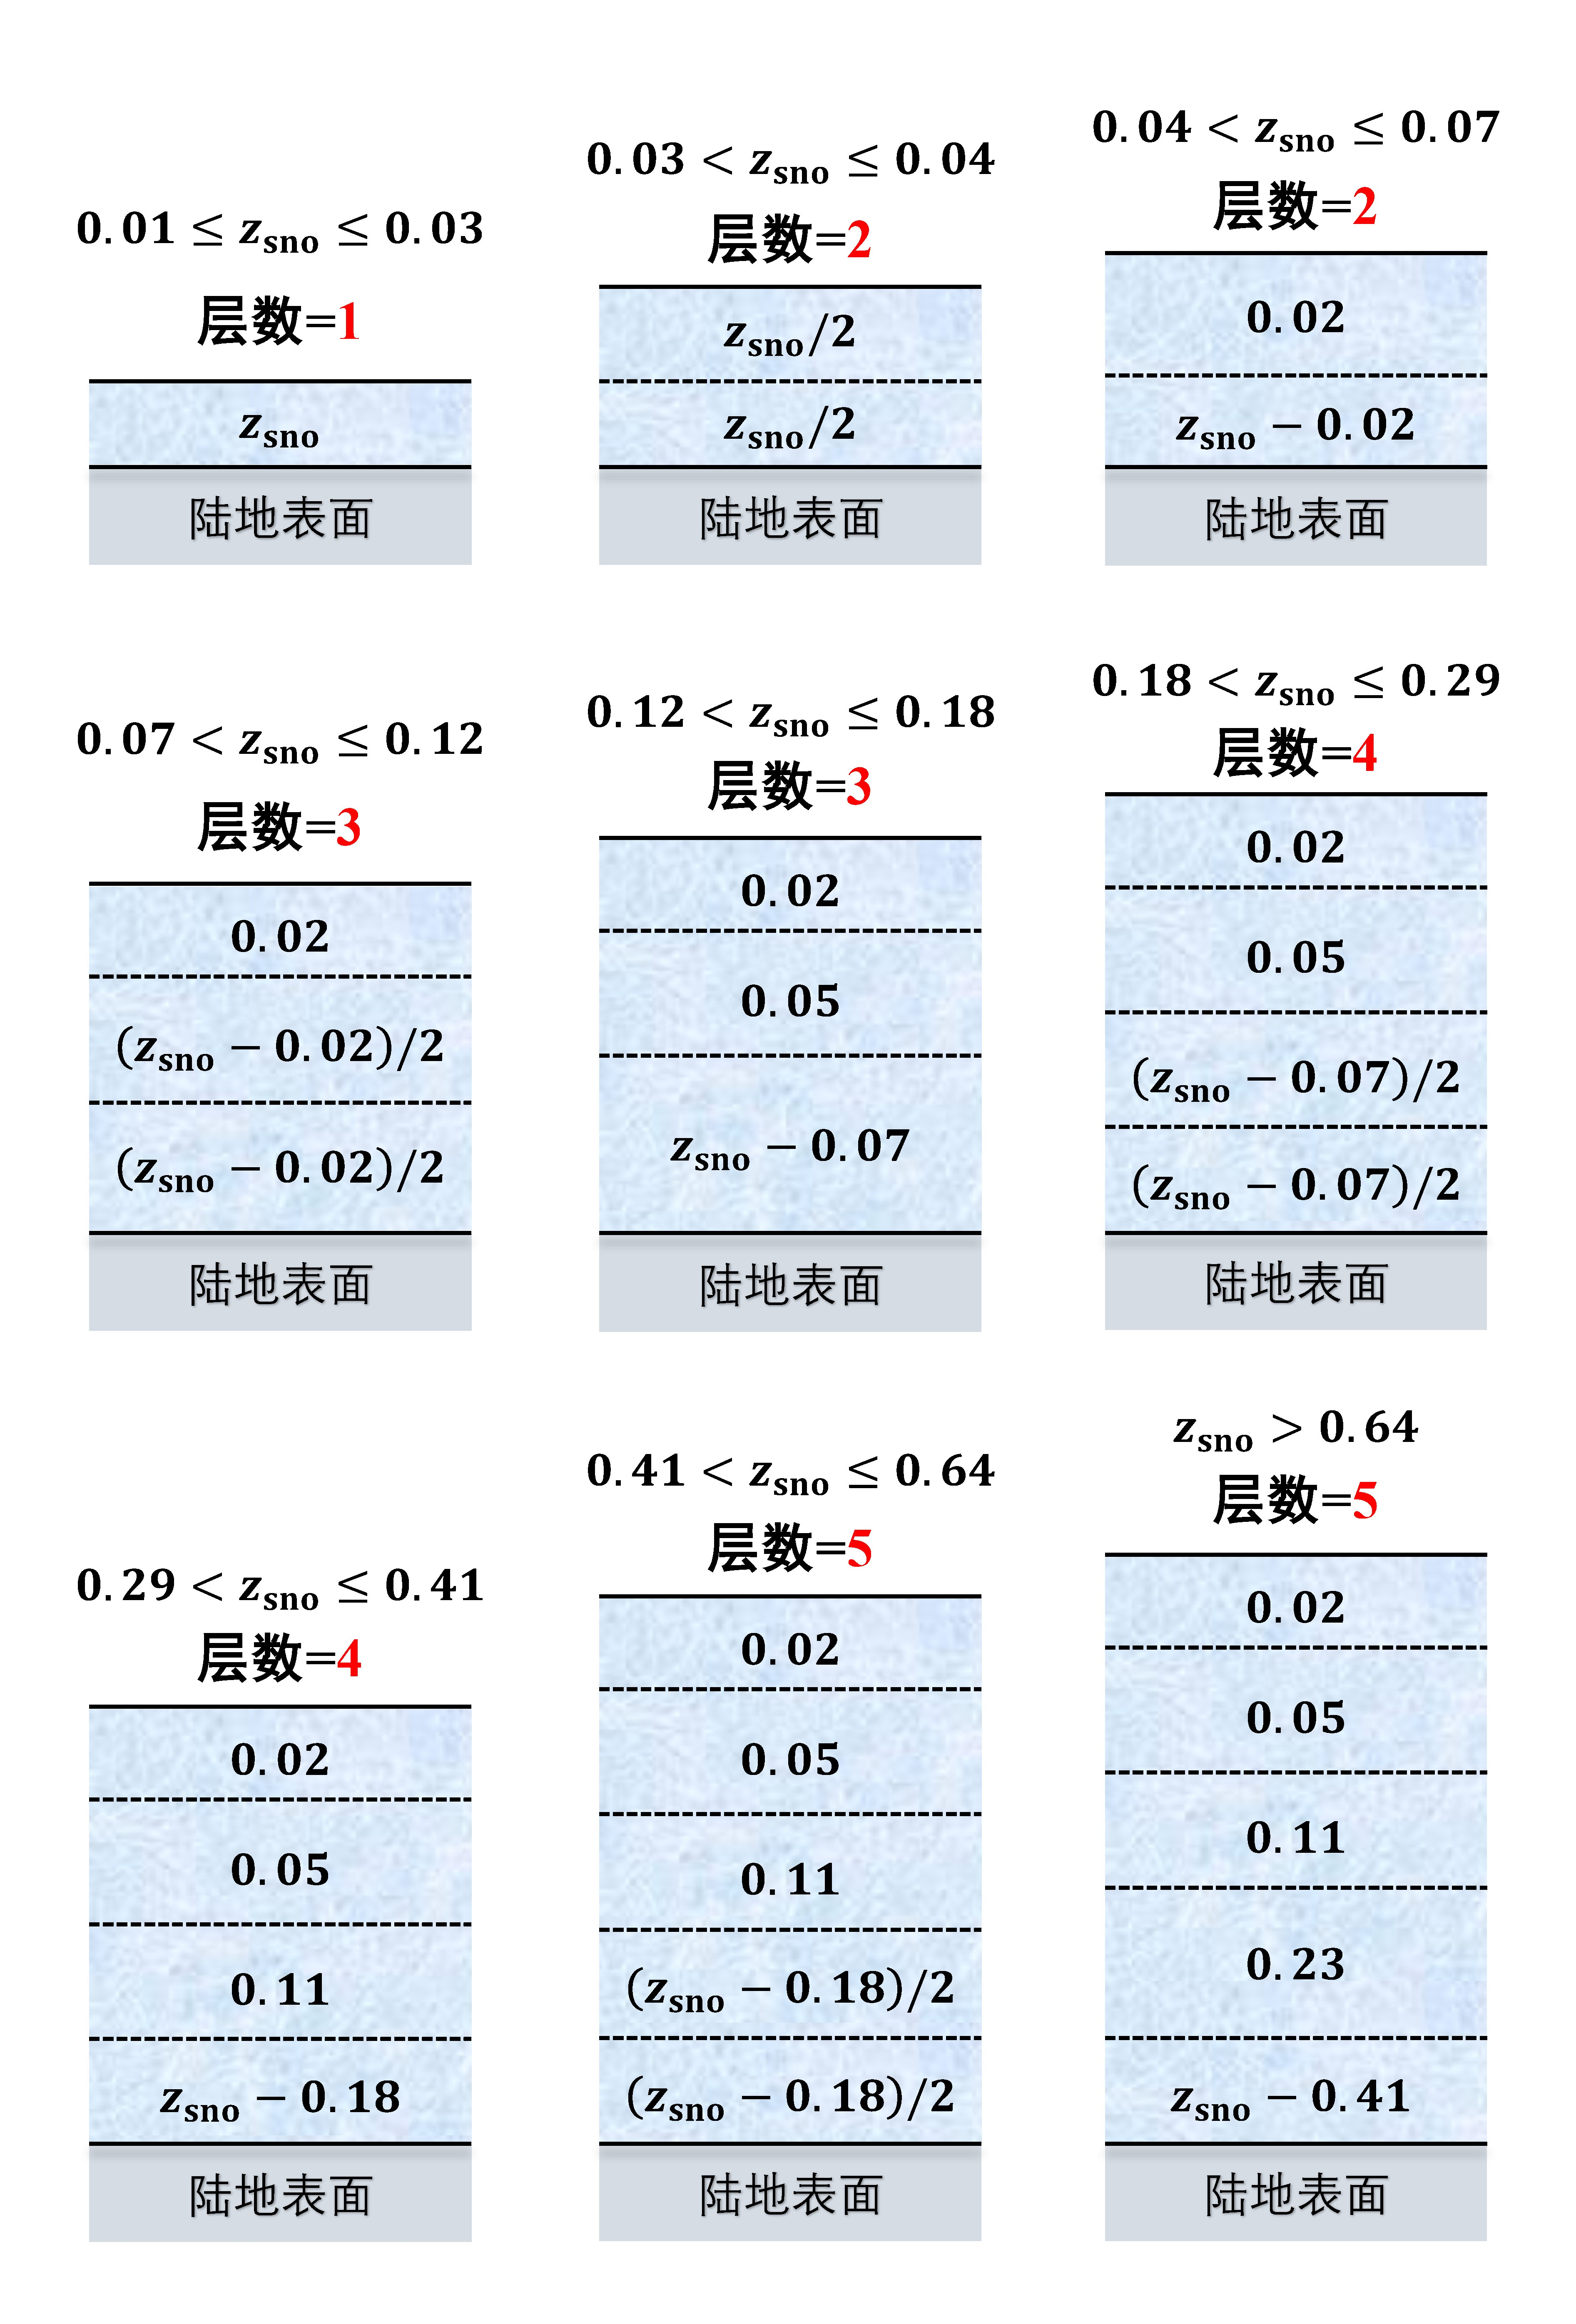
\includegraphics[width=0.8\textwidth]{Figures/模式构架/积雪分层.jpg}
\caption[CoLM积雪分层方案]{CoLM积雪分层方案。当$z_{sno}<0.01$时不形成积雪层}
\label{fig:积雪分层}
\end{figure}
}
    
$z_{h,0}=0$为雪盖底层与土壤表层交界处的高度,$\Delta z_{i}$为第$i$层积雪的厚度。将交界面以上的高度定义为负值,则每一层雪的中心高度$z_i$~(m)与相邻两层雪交界处的高度$z_{h,i}$~(m)计算为:
\begin{equation}
\begin{aligned}
z_{i} &= z_{h, i}-0.5 \Delta z_{i} \quad i=0, \ldots, snl+1 \\ 
z_{h, i} &= z_{h, i+1}-\Delta z_{i+1}  \quad i=-1, \ldots, snl
\end{aligned}
\end{equation}


\section{计算框架}\label{计算框架}

{
\begin{figure}[htbp]
\centering
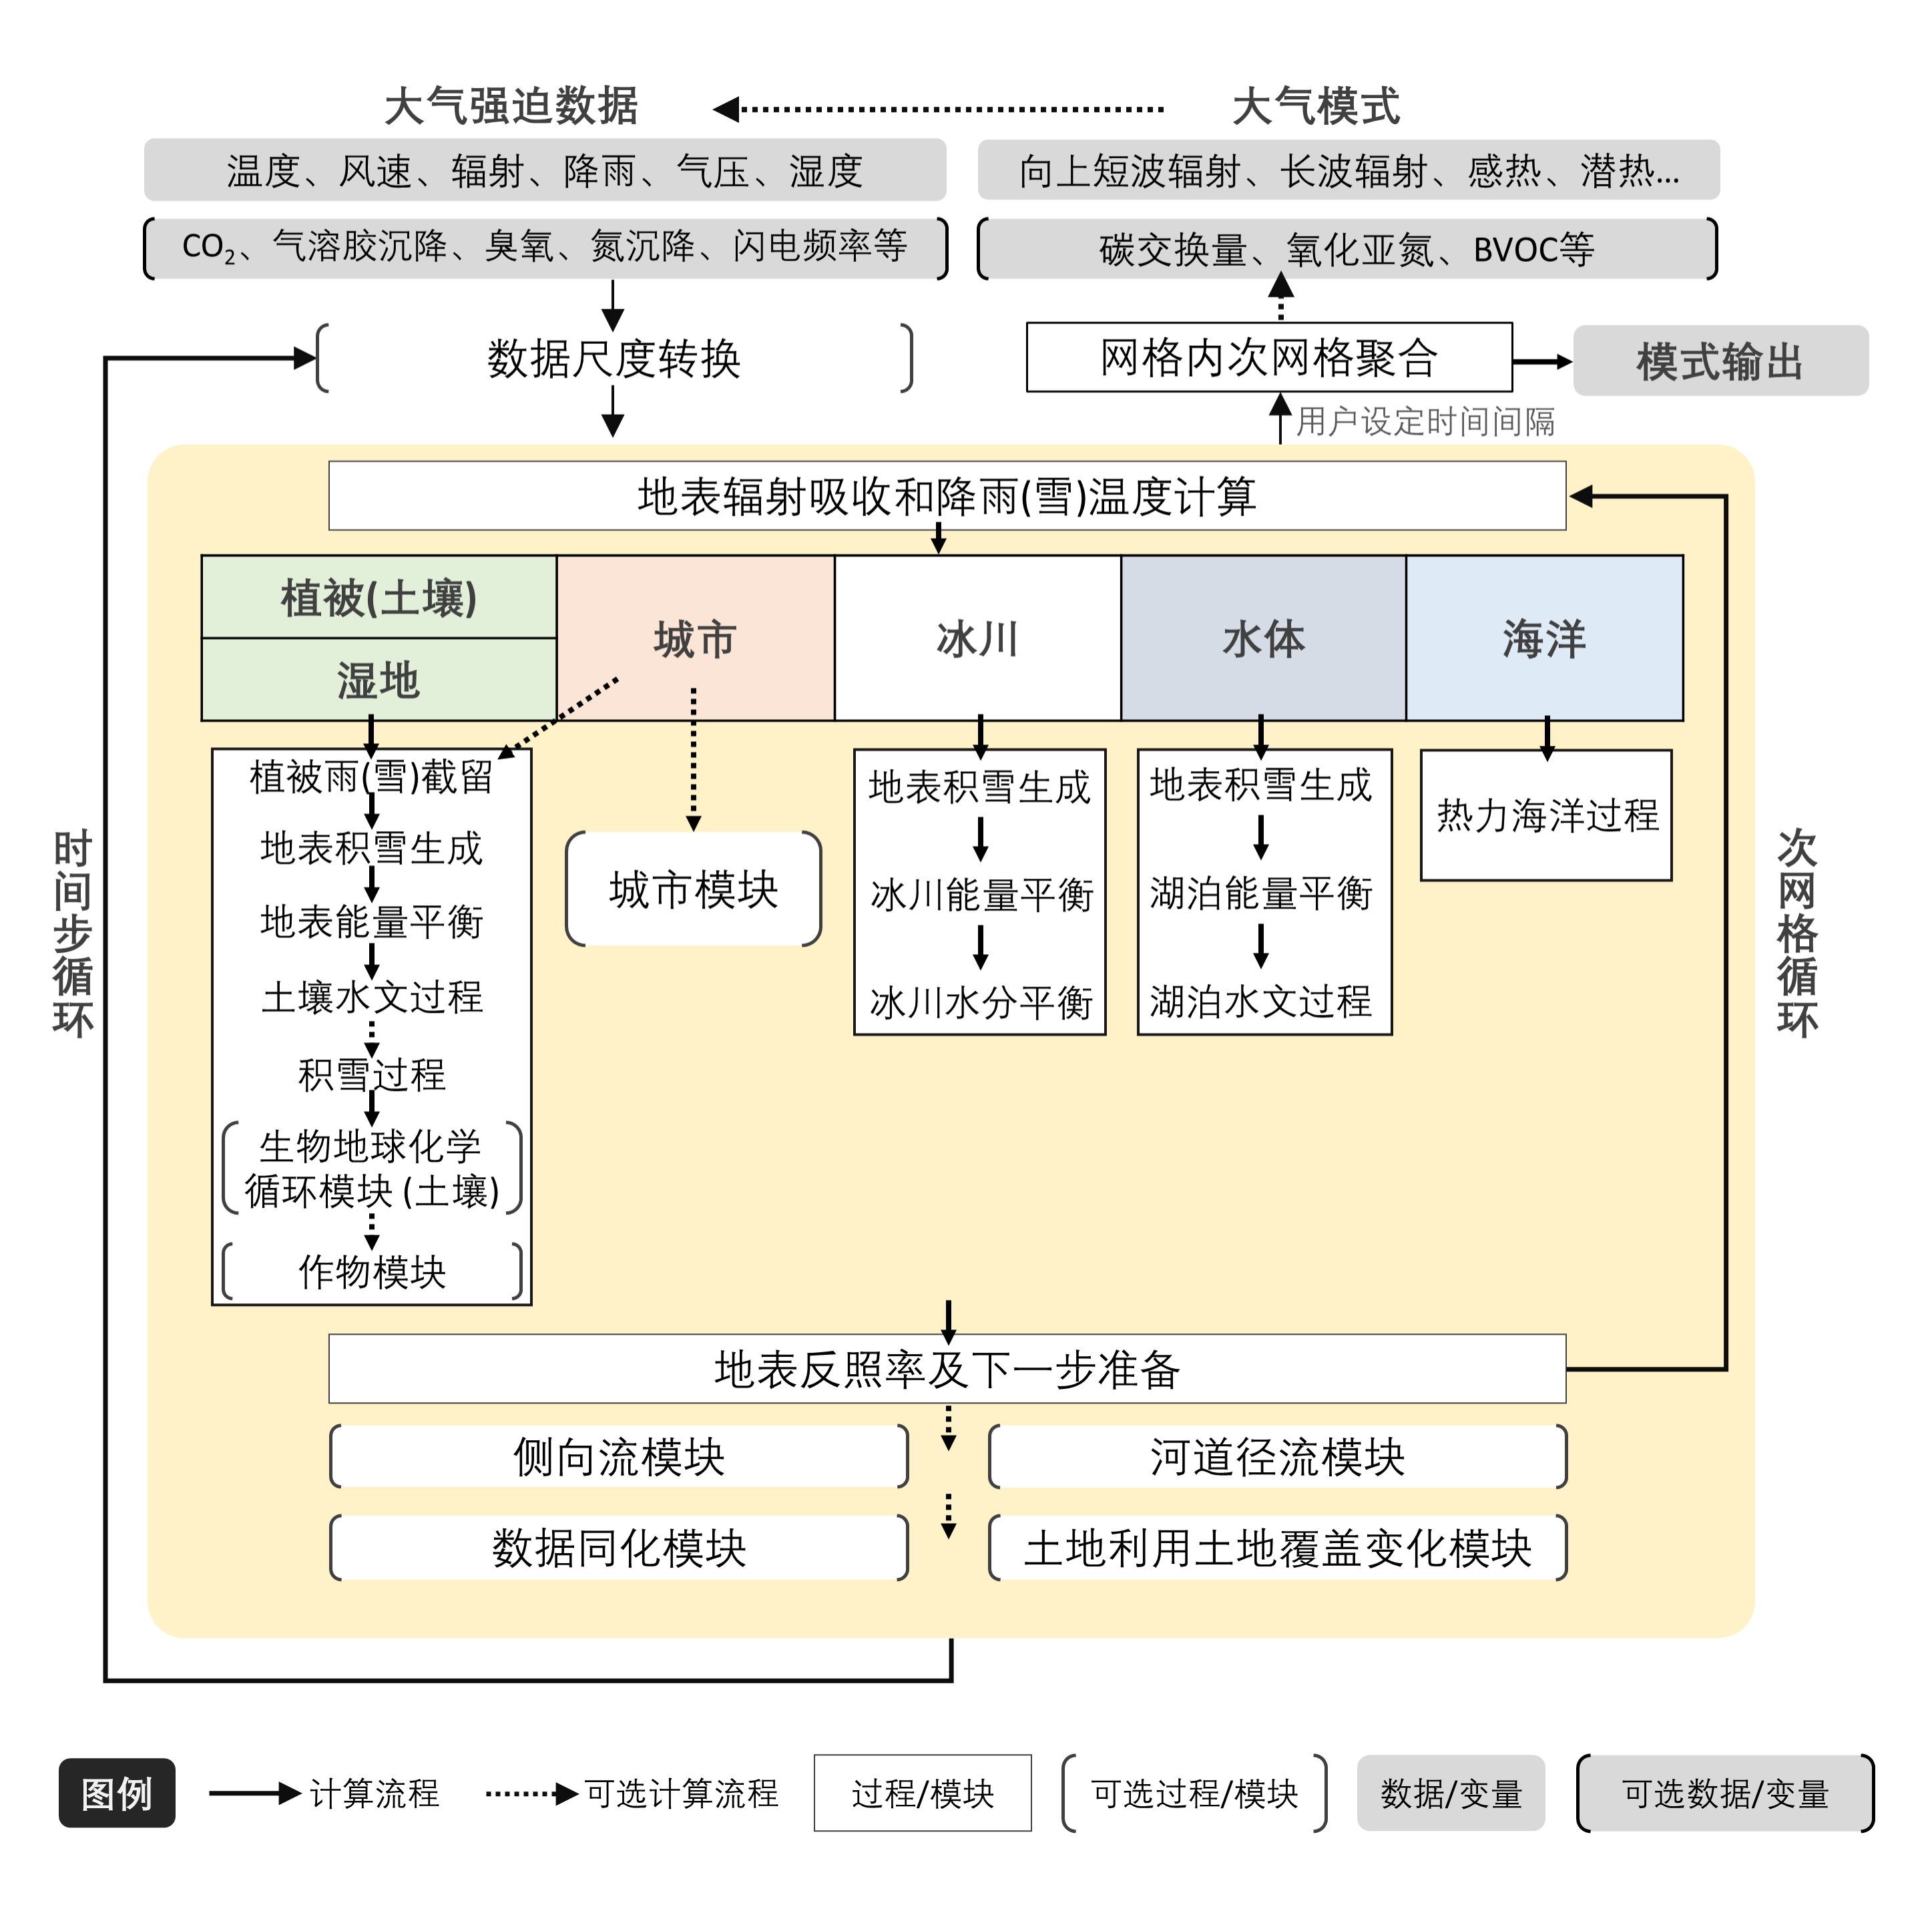
\includegraphics[width=\textwidth]{Figures/模式构架/CoLM计算框图_v5.png}
\caption{CoLM计算框图}
\label{fig:CoLM计算框图}
\end{figure}
}

CoLM主程序计算流程主要包括模式数据的读取,时间步循环,次网格循环,以及模式数据输出(图~\ref{fig:CoLM计算框图})。涉及的过程主要在\texttt{main}文件夹下\texttt{CoLM.F90},\texttt{CoLMDRIVER.F90}及 \allowbreak \texttt{CoLMMAIN.F90}
\allowbreak (\texttt{URBAN\allowbreak /Urban\allowbreak \_CoLMMAIN.F90},当城市模式打开时)文件中进行调用。

\textbf{模式数据读取}大概可分为驱动数据和地表数据。其中驱动数据可以通过在离线模式下读取大气强迫数据,包括温度、风速、辐射、降雨等必要变量,以及气溶胶、氮沉降等可选变量,具体可参见表~\ref{tab:陆面模式所需的大气状态变量}。目前可用于驱动CoLM离线运行的大气驱动数据集详见表~\ref{tab:可用于驱动CoLM离线运行的大气驱动数据集}。在读取过程中可根据需要进行适当数据尺度转换(章节~\ref{大气强迫降尺度});如时间尺度不匹配,可进行简单时间维插值,详见\hyperlink{驱动数据时间尺度插值}{驱动数据时间尺度插值};另外,驱动数据可以通过与大气模式耦合来获得(章节~\ref{CoLM与大气模式耦合})。

\textbf{模式数据输出}可通过既定的网格在用户设定的时间间隔内进行变量聚合(次网格聚合到网格,章节~\ref{次网格}),作为模式运行结果输出(history file)或者对耦合大气模式的反馈,具体可参见表~\ref{tab:大气模式所需的陆面模式输出变量}。网格输出类型包括经纬度网格、流域单元网格(章节~\ref{流域单元网格})及非结构网格(章节~\ref{非结构网格}),同时也可以根据用户需求进行网格转换。地表数据涉及的内容繁多,根据模式运行所选择的功能选项按需读取,涉及的数据详见章节~\ref{基础数据} \nameref{基础数据}部分。

\textbf{时间步循环}主要包括次网格循环(涉及的过程在\texttt{CoLMDRIVER.F90}和\texttt{CoLMMAIN.F90\allowbreak /Urban\allowbreak \_CoLMMAIN.F90}进行调用)以及可选模块(侧向流、河道径流、数据同化和土地利用土地覆盖变化等模块,在\texttt{CoLM.F90}进行调用)的运行(图~\ref{fig:CoLM计算框图} \textbf{时间步循环}所示)。

\textbf{次网格循环}沿用了原CoLM运行方式,对5种非海洋patch进行循环计算,即植被(含裸土)、城市、湿地、冰川和水体。如果打开海洋模块,则在循环中加入对海洋热力过程的模拟(图~\ref{fig:CoLM计算框图} \textbf{次网格循环}所示)。图中\textbf{次网格循环}所列过程为其简要列表,具体物理过程将从\nameref{part:flux}、\nameref{part:temp}、\nameref{part:SPC}、\nameref{part:hydro}、\nameref{part:BGC}、\nameref{part:human}、\nameref{part:scaling}七大部分各相关章节进行阐述。

\section{陆气耦合}\label{陆气耦合}
\subsection{陆面模式与大气模式的数据交换}
陆面模式的运行需要当前时刻的大气状态作为驱动。当陆面模式离线运行时(offline),大气状态可由观测数据、再分析数据或大气模式模拟结果数据直接提供;当陆面模式置于天气/气候/地球系统模式耦合运行时(online),大气状态可由大气模式通过耦合器或程序调用接口实时传递给陆面模式。陆面模式接收到当前时刻的大气状态后,首先结合上一时刻的植被、雪盖或土壤的状态和地表特征(如地表反照率、空气动力学阻抗等)计算当前时刻的陆气湍流交换通量、辐射通量、进入地表的能量和水分通量等,然后基于这些通量条件计算当前时刻的植被、雪盖或土壤的状态变量和地表特征量。在耦合运行时,这些地表通量和状态变量实时返回给大气,为大气模式进行下一时刻的计算提供下边界条件。陆面模式所需的大气变量和大气模式所需的陆面变量详见表~\ref{tab:陆面模式所需的大气状态变量} 和表~\ref{tab:大气模式所需的陆面模式输出变量}。

关于参考高度(reference height) (见表~\ref{tab:陆面模式所需的大气状态变量}),即大气驱动变量所在的高度,需要做一点特殊说明。参考高度的设置通常比较随意,一般认为只要不超过近地层即可。在陆面模式离线运行试验中,参考高度通常为10 m到50 m的高度;在陆气耦合试验中,参考高度通常设为大气模式的最底层。但本团队的最新研究\citep{liu2023referenceheight} 表明,把参考高度设置在近地层顶附近,可以显著提高地表湍流通量的模拟精度。考虑1 km的典型对流边界层高度,建议参考高度设置为100 m左右。

{
\begin{table}[htbp]
\centering
\caption{陆面模式所需的大气状态变量}
\label{tab:陆面模式所需的大气状态变量}
\begin{threeparttable}
\begin{tabular}{lcc}
\toprule
大气状态变量               & 变量名           & 单位           \\  \midrule
大气风速参考高度             & $z_{atm,m}$   & m            \\
大气温度参考高度             & $z_{atm,h}$   & m            \\
大气比湿参考高度             & $z_{atm,w}$   & m            \\
位于$z_{atm,m}$高度的纬向风速 & $u_{atm}$     & \unit{m.s^{-1}}   \\
位于$z_{atm,m}$高度的经向风速 & $v_{atm}$     & \unit{m.s^{-1}}   \\
位于$z_{atm,h}$高度的大气温度 & $T_{atm}$     & K            \\
位于$z_{atm,w}$高度的大气比湿 & $q_{atm}$     & \unit{kg.kg^{-1}} \\
近地面气压                & $P_{atm}$     & Pa           \\
近地面下行长波辐射            & $L ^\downarrow$ & \unit{W.m^{-2}}   \\
近地面下行短波辐射            & $S ^\downarrow$ & \unit{W.m^{-2}}   \\
降水                   & $p$           & \unit{mm.s^{-1}}      \\
二氧化碳浓度               & $c_a$         & ppmv         \\
臭氧浓度                 & $c_o$         & \unit{mol.mol^{-1}}  \\
大气气溶胶沉降速率        & $D_{sp}$      & \unit{kg.m^{-2}.s^{-1}}  \\
氮沉降速率                & $N_{dep}$     & \unit{g(N).m^{-2}.yr^{-1}}   \\
闪电频率                 & $I_l$         & \unit{flash.km^{-2}.hr^{-1}} \\ \bottomrule    
\end{tabular}
\begin{tablenotes}
\footnotesize
\item[1] 根据气溶胶种类和亲水性,气溶胶沉降速率可按照14种不同的气溶胶给出,其中沙尘气溶胶可分为8种(视为4种不同气溶胶颗粒大小的干气溶胶或湿气溶胶),黑碳气溶胶分为3种(干亲水性气溶胶、湿亲水性气溶胶、干疏水性气溶胶),有机碳气溶胶分为3种(干亲水性气溶胶、湿亲水性气溶胶、干疏水性气溶胶)。气溶胶沉降主要用于积雪、冰盖和气溶胶辐射模型 (SNICAR),影响积雪反照率和积雪内部辐射传输过程的计算。 
\item[2] 氮沉降速率用于生物地球化学循环模型(BGC),表征无机氮(主要由氮氧化物 $\mathrm{NO_y}$ 和氮氢化物 $\mathrm{NH_x}$ 组成)在陆地表面的沉降通量。
\item[3] 臭氧浓度用于模拟其对气孔导度等植被生理过程的影响,闪电频率用于火灾模式。
\end{tablenotes}
\end{threeparttable}
\end{table}
}
{
\begin{table}[htbp]
\centering
\caption{大气模式所需的陆面模式输出变量}
\label{tab:大气模式所需的陆面模式输出变量}
\begin{threeparttable}
\begin{tabular}{lcc}
\toprule
陆面模式输出变量    & 变量名                            & 单位      \\ \midrule
潜热通量        & $\lambda E$ & \unit{W.m^{-2}}    \\
感热通量        & $H$                    & \unit{W.m^{-2}}    \\
水汽通量        & $E$                    & \unit{mm.s^{-1}}    \\
纬向动量通量      & $\tau_{x}$      & \unit{kg.m^{-1}.s^{-2}} \\
经向动量通量      & $\tau_{y}$      & \unit{kg.m.s^{-2}} \\
地表出射长波辐射通量  & $L ^\uparrow$    & \unit{W.m^{-2}}    \\
直射光可见光波段反照率 & $\alpha_{vis,dir}$             & -       \\
直射光近红外波段反照率 & $\alpha_{nir,dir}$             & -       \\
漫射光可见光波段反照率 & $\alpha_{vis,dif}$             & -       \\
漫射光近红外波段反照率 & $\alpha_{nir,dif}$             & -       \\
地表辐射温度      & $T_{rad}$                      & K       \\
近地面2 m温度     & $T_{2m}$                       & K       \\
近地面2 m比湿     & $q_{2m}$                       & \unit{kg.kg^{-1}}   \\
近地面10 m风速    & $u_{10m}$                      & \unit{m.s^{-1}}     \\
雪水当量        & $W_{sno}$                      & mm      \\
空气动力学阻抗     & $r_{am}$                       & \unit{s.m^{-1}}     \\
摩擦速度        & $u_\ast$                       & \unit{m.s^{-1}}     \\
净生态系统碳交换通量  &   NEE                      & \unit{g.C.m^{-2}.s^{-1}} \\
氧化亚氮浓度      & $\mathrm{N_2O}$               & \unit{g.N.m^{-2}.s^{-1}}\\
\bottomrule         
\end{tabular}
\begin{tablenotes}
\footnotesize
\item[1] $\lambda$ 表示蒸发潜热(\unit{J.kg^{-1}}),$\lambda$ 根据地表水份是否冻结取为蒸发潜热或升华潜热。
\end{tablenotes}
\end{threeparttable}
\end{table}
}


\subsection{离线运行CoLM可使用的大气驱动数据集}\label{离线大气驱动数据集}
CoLM支持多套大气驱动数据集的使用,包括全球/区域格点数据和单点数据。其中,全球/区域格点数据见表~\ref{tab:可用于驱动CoLM离线运行的大气驱动数据集}。用户也可使用其他数据,只需参照任意一种目前支持的数据集制作成对应的数据格式,并参照该数据对应的namelist提供相应的信息即可使用。特别地,当运行区域或单点模式时,大气驱动数据可选择任意一套覆盖该区域或该点的数据,模式可自动从大气驱动数据中提取出该区域或该点的数据信息来驱动CoLM。

\hypertarget{驱动数据时间尺度插值}{CoLM默认的积分时间步长为1800秒}。当大气驱动数据的时间分辨率不满足这一积分步长时,相邻数据之间将进行插值以保持大气驱动数据的时间分辨率与积分步长相同。其中,温度、气压、比湿、风速、长波辐射通量默认采用线性插值获得,降水速率采用临近时刻插值获得,短波辐射通量采用基于太阳高度角的余弦值加权平均获得。短波辐射通量的插值具体操作为:对于插值时刻$t_M$,短波辐射通量$S^{\downarrow}$($t_M$)计算为
\begin{equation}\label{t_M}
S^{\downarrow}\left(t_{M}\right)=\left\{\begin{array}{ll}\frac{ \mu\left(t_{M}\right)}{\overline {\sum_{i=1}^{\frac{\Delta t_{FD}}{\Delta t_{M}}} \mu\left(t_{M_{i}}\right)}}S^{\downarrow}\left(t_{F D}\right)  & \text { 当 }\ \mu\left(t_{M}\right)>0.001 \\
0 & \text { 当 }\ \mu\left(t_{M}\right) \leqslant 0.001\end{array}\right.
\end{equation}
其中,$\Delta t_{FD}$代表驱动数据的时间间隔(例如,对于3-hourly数据$\Delta t_{FD}$=10800秒),$\Delta t_{M}$代表模式积分步长,$S^{\downarrow}(t_{FD})$ 代表比$t_M$时刻早的最接近$t_M$时刻的短波辐射驱动数据,$\mu\left(t_M\right)$代表$t_M$时刻的太阳高度角的余弦值,$\overline{
\sum_{i=1}^{\frac{\Delta t_{F D}}{\Delta t_{M}}} \mu\left(t_{M_{i}}\right)}$代表落在驱动数据时间间隔内的所有模式积分时刻的太阳高度角余弦值的平均值。以上插值方式可根据原数据特征及用户需求在大气强迫namelist配置文件中进行修改。

当大气强迫只有总的入射太阳辐射时,CoLM采用源于Sib2的经验方法对其进行直射/漫射,可见光/近红外分解。根据网格所在经纬度和Julian
day计算太阳高度角余弦值\(\mu\),由此计算云覆盖比例:
%
\begin{equation}
f_{cloud} = \min\left( 1,\max\left( 0.58,\frac{1160\mu - S^{\downarrow}}{963\mu} \right) \right)
\end{equation}
%
入射漫射辐射比例首先计算为:
%
\begin{equation}
f_{dif} = \min\left( 1,\max\left( 0,\frac{0.0604}{\mu - 0.0223} + 0.0683 \right) \right)
\end{equation}
%
然后根据云覆盖比例调整为:
%
\begin{equation}
f_{dif} = f_{dif} + \left( 1 - f_{dif} \right)f_{cloud}
\end{equation}
%
太阳辐射可见光波段占比计算为:
%
\begin{equation}
f_{vis} = \frac{500 - {464f}_{cloud}}{\left( 580 - {499f}_{cloud} \right) + \left( 580 - {464f}_{cloud} \right)}
\end{equation}
%
最终分波段的直射/漫射入射太阳辐射计算为:
%
\begin{equation}
\begin{aligned}
S_{vis,dir}^{\downarrow} &= S^{\downarrow}\left( 1 - f_{dif} \right)f_{vis}\\
%
S_{nir,dir}^{\downarrow} &= S^{\downarrow}\left( 1 - f_{dif} \right)\left( 1 - f_{vis} \right)\\
%
S_{vis,dif}^{\downarrow} &= S^{\downarrow}f_{dif}f_{vis}\\
%
S_{nir,dif}^{\downarrow} &= S^{\downarrow}f_{dif}\left( 1 - f_{vis} \right)
\end{aligned}
\end{equation}
%

对于QIAN强迫驱动太阳辐射,CoLM采用CLM4.5方案,可见光和近红外分配系数$f_{vis}=f_{nir}=0.5$。对于以上两个波段,太阳辐射被进一步分为直射光与漫射光。直射光在可见光波段的比例系数为
\begin{equation}\label{R_vis}
f_{vis,dir}=a_{0}+a_{1} f_{vis} S^{\downarrow}+a_{2}(f_{vis} S^{\downarrow})^{2}+a_{3}(f_{vis} S^{\downarrow})^{3} \quad 0.01 \leqslant f_{vis,dir} \leqslant 0.99
\end{equation}
直射光在近红外波段的比例系数为
\begin{equation}
f_{nir,dir}=b_{0}+b_{1}(1-f_{nir}) S^{\downarrow}+b_{2}((1-f_{nir}) S^{\downarrow})^{2}+b_{3}((1-f_{nir}) S^{\downarrow})^{3} \quad 0.01 \leqslant f_{nir,dir} \leqslant 0.99
\end{equation}
其中$a_0$=0.17639, $a_1$=0.0038, $a_2=-9.0039\times{10}^{-8}$, $a_3=8.1351\times10^{-9}$, $b_0=0.29548$, $b_1=0.00504$, $b_2=-1.4957\times10^{-5}$, $b_3=1.4881\times10^{-8}$。这些系数来自对 NCAR-CAM 模式模拟结果的拟合。
相应分波段的直射/漫射入射太阳辐射计算为:
%
\begin{equation}
\begin{aligned}
S_{vis,dir}^{\downarrow} &= S^{\downarrow}f_{vis,dir} f_{vis}\\
%
S_{nir,dir}^{\downarrow} &= S^{\downarrow}f_{nir,dir} f_{nir} \\
%
S_{vis,dif}^{\downarrow} &= S^{\downarrow}\left ( 1 - f_{vis,dir} \right ) f_{vis}\\
%
S_{nir,dif}^{\downarrow} &= S^{\downarrow}\left ( 1 - f_{nir,dir} \right ) f_{nir}
\end{aligned}
\end{equation}

当大气驱动数据未提供下行长波辐射通量时,模式将根据大气温度$T_{atm}$、比湿$q_{atm}$和水汽压$e_{atm}$计算获得~\citep{idso1981SetEquationsFull},计算方案为
\begin{equation}\label{L_downarrow}
L ^\downarrow=\left[0.70+5.95 \times 10^{-5} \times 0.01 e_{a t m} \exp \left(\frac{1500}{T_{a t m}}\right)\right] \sigma T_{a t m}^{4}
\end{equation}
其中大气水汽压计算为$e_{a t m}=\frac{P_{a t m} q_{a t m}}{0.622+0.378 q_{a t m}}$,$\sigma$为Stefan-Boltzmann常数。

未来情景下的大气驱动数据可采用CMIP6气候模式的模拟输出结果。当历史时期与未来情景共同模拟时,未来时期CMIP6气候模式的模拟结果往往不能直接使用,因为当模拟历史时期使用的大气驱动数据来自观测或再分析数据时,其均值、时空变率、数据拼接时刻的取值与CMIP6气候模式的模拟结果往往存在较大差异。这里可使用异常值叠加方式来融合历史与未来的大气驱动数据。举例说明:当模拟1850--2099年的陆面状态时,1850--2014年的历史时期模拟可采用GSWP3大气驱动数据,2015--2099年的未来时期模拟可采用CMIP6气候模式的模拟结果,两套数据的融合方式如下:首先,将2015--2100年各驱动变量的逐月数据去除气候态的季节循环,得到带有某种社会经济排放情景下的各驱动变量的异常值序列,此序列可表征未来气候变化趋势的影响;其次,将历史时期有限时间段的各大气驱动变量反复叠加到未来时期各驱动变量的异常值序列(例如将2010-2014年的大气驱动数据反复叠加到2015--2019、2020--2024、…、2095--2099年的异常值序列),得到可使用的未来时期的大气驱动数据。此种数据融合方式既得到了未来时期的气候变化趋势,又保留了历史时期大气驱动数据的年际变率,缩小了历史时期与未来时期数据拼接时刻的数据阶跃程度。对于不同的大气驱动变量,历史时期数据与未来时期异常值序列的叠加方式不同:对于温度、气压、比湿、风速等大气状态变量,叠加方式采用加法叠加($S_{new}=S_{old}+k_{anomaly}$),对于降水、下行短波辐射通量、下行长波辐射通量,叠加方式采用乘法叠加($F_{new}=F_{old}\times k_{anomaly}$)。


最后,针对单点模拟,CoLM已经收集整理测试的站点信息见表~\ref{tab:CoLM离线运行已经测试的站点列表}。

\subsection{通过耦合器实现CoLM与大气模式的耦合模拟}\label{CoLM与大气模式耦合}
陆面是天气/气候/地球系统的重要组成部分,其物理、化学、生物过程深刻影响着陆地与大气、陆地与海洋之间的能量与物质交换~\citep{Dai2020}。因此,在天气/气候/地球系统模式的耦合框架下运行陆面过程模式,既可刻画在特定条件下陆面系统内部复杂的多圈层多尺度过程,又可将陆面系统变化反馈给大气和海洋系统,充分刻画地球系统各分量之间紧密的相互作用。

地球系统模式通过耦合器连接大气、海洋、陆面、海冰等多个分量模式,形成一个包含地球系统各圈层演化和相互作用过程的完整模式软件。耦合器负责多个分量模式之间的数据交换、不同网格之间数据的插值、以及物质能量等的守恒性诊断,并控制整个地球系统模式的积分模拟~\citep{tangyanli_2015, chenyiran_2017}。耦合器的“可插拔式”框架更有利于促进地球系统模式的模块化和高效并行化。现有的耦合器主要有美国国家大气研究中心(National Center For Atmospheric Research, NCAR)开发的CPL (Coupler)耦合器、美国普林斯顿大学地球物理流体动力学实验室(Geophysical Fluid Dynamics Laboratory)开发的FMS (Flexible Modelling System)、美国的耦合工具库ESMF(Earth System Modelling Framework)、法国欧洲气候模拟和全球变化研究中心开发的OASIS等,其中美国NCAR的CPL和法国的OASIS应用最为广泛。近年来,国内自主研发的耦合器得到了显著发展,其中由清华大学研制的耦合器C-Coupler取得了一系列自主创新,完成了三个版本的研制~\citep{LiuLi_2023},并逐渐成长为国际首个面向地球系统数值预报的一体化软件平台,已稳定应用于国内多家业务和科研单位。目前,CoLM已经通过CPL7实现与中国科学院地球系统模式CAS-ESM和区域气候模式CWRF的耦合,使得CoLM成为其中的陆面分量模式。其他使用CPL7的地球系统模式可通过类似流程实现与CoLM的耦合。CoLM将在后续尝试通过国产耦合器C-Coupler实现与中国气象局全球数值天气预报系统CMA-GFS等更多国内业务预报模式的耦合,使得CoLM能够更好地服务于我国天气气候研究与业务预报,有效提升天气气候模拟与预测精度。本节将简要介绍CoLM与CPL7的基本耦合原理,CoLM与CAS-ESM和CWRF的耦合流程见附录。

CPL7作为目前使用最为广泛的耦合器之一,其功能不再仅局限于地球系统模式中不同分量模式的数据连通器,它可直接作为模式的顶层驱动,控制各个分量模式运行的先后次序。CPL7作为总控程序控制CAS-ESM的运行流程可参见图~\ref{fig:CAS-ESM的运行流程},其中每个分量模式均需进行初始化,之后从耦合器读入需要的数据、运行模式、将必要的运行结果发送回耦合器,以此流程逐步积分直至结束。CPL7通过标准代码接口调用各个分量模式的初始化、运行和结束子程序,并在分量模式需要进行数据交换时调用耦合器函数(网格插值、数据发送与接收、重排与融合、通量计算等)实现分量模式之间的相互作用。分量模式之间的并发关系可根据模式计算量和用户需求来指定。总体上,CPL7实现总控调度和各分量模式之间的耦合主要基于三个方面的设计:并行机制、网格映射和时间管理。下面对这三方面逐一进行简要介绍。
{
\begin{figure}[htbp]
\centering
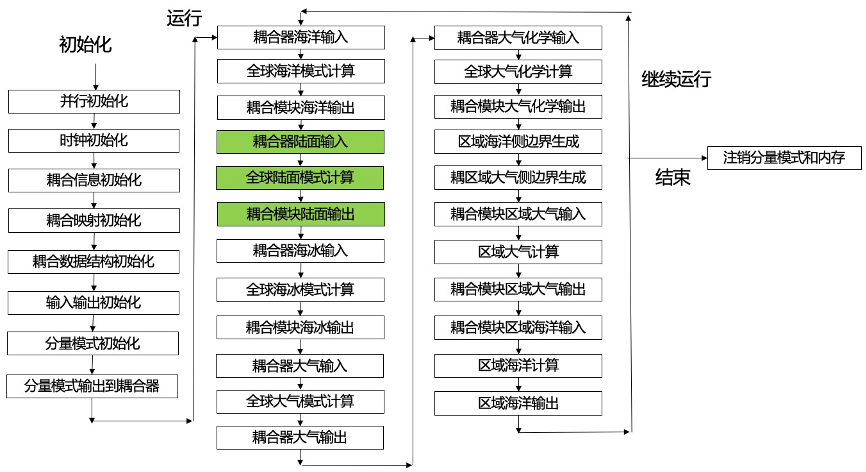
\includegraphics{Figures/模式构架/CAS-ESM的运行流程.png}
\caption[CPL7作为总控程序控制CAS-ESM的运行流程]{CPL7作为总控程序控制CAS-ESM的运行流程(引自何卷雄关于“地球系统数值模拟装置项目地球系统模式数值模拟系统集成模块分系统培训”PPT)}
\label{fig:CAS-ESM的运行流程}
\end{figure}
}

首先,在模式并行机制方面,CPL7除了将地球系统模式整体划分为一个完整的通讯域外,每个分量模式自身以及分量模式与耦合器各形成两个子通讯域,见图~\ref{fig:CPL7并行机制示意图}。每个分量模式自身的通讯域用于模式内部的数据交换,它使得分量模式各自的并行算法得以保持,不受其他分量模式和耦合环境的影响。每个分量模式与耦合器形成的通讯域用于模式与耦合器的数据交换,各分量模式只能从耦合器获取运行时所需的数据,并将其他分量模式所需的数据直接发送给耦合器,这种由耦合器充当数据传输枢纽的方式使得数据传递变得易于管理,有效避免了以往各分量模式之间进行数据传递时由于数据分辨率和所在处理器不同造成的混乱。基于此,当CoLM与CPL7进行耦合时,CoLM可直接接收CPL7提前划分的用于陆面模式独立运行的通讯域,并通过CPL7的模型耦合工具MCT(The Model Coupling Toolkit)提供的数据结构Attrvect实现与CPL7的数据交换。

{
\begin{figure}[htbp]
\centering
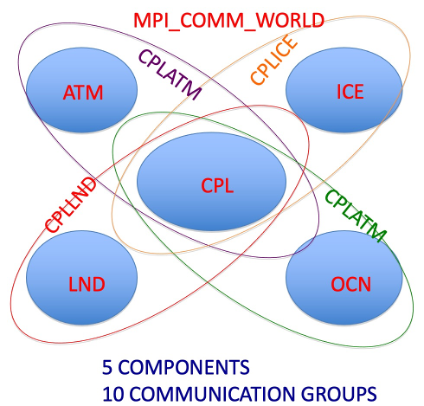
\includegraphics{Figures/模式构架/CPL7并行机制示意图.png}
\caption[CPL7并行机制示意图]{CPL7并行机制示意图。对于有5个组件(大气、陆面、海洋、海冰和耦合器)组成的地球系统模式,共划分为10个通讯域:5个组件各自形成通讯域、4个分量模式分别与耦合器形成通讯域、以及5个组件整体形成一个通讯域(引自何卷雄关于“地球系统数值模拟装置项目地球系统模式数值模拟系统集成模块分系统培训”PPT)}
\label{fig:CPL7并行机制示意图}
\end{figure}
}

其次,在网格映射方面,CPL7实现网格映射主要依赖模型耦合工具。目前,CPL7支持的模型耦合工具有MCT和地球系统模拟框架软件ESMF,默认情况下使用MCT。MCT提供的数据结构见图~\ref{fig:MCT的基本数据结构}。其中,GlobalSegmentMap主要描述各分量模式局部网格在全局网格上的映射,存储的信息包括分量模式的ID号、有多少个数据段和全局网格、每个数据段的网格在全局中的起始编号和长度、以及每个数据段所属的处理器编号,通过以上信息可获得各分量模式在每个处理器上处理的局部网格与全局网格的对应关系,此对应关系用于分量模式与耦合器进行数据交换时,数据在耦合器中的重新排列。GeneralGrid存储了各分量模式的物理网格信息,包含了每个处理器的网格坐标、面积、海陆标识、及其在全球网格的编号等。AttrVect是GeneralGrid数据结构中的一部分,它是一个二维数组,用于存储各分量模式在每个处理器的所有格点上需要进行交换的物理量数据,并与耦合器进行通信。GlobalSegmentMap和GeneralGrid是分量模式与耦合器进行数据交换的最基本的数据结构。当CoLM与CPL7进行耦合时,需要对GlobalSegmentMap和GeneralGrid进行相应信息的赋值,才能实现二者的信息交换。

{
\begin{figure}[htbp]
\centering
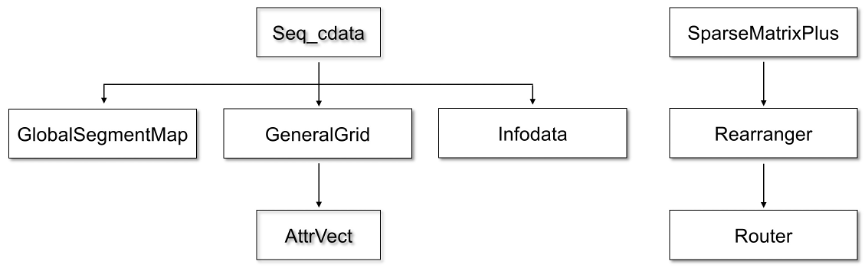
\includegraphics{Figures/模式构架/MCT的基本数据结构.png}
\caption{模型耦合工具MCT使用的基本数据结构}
\label{fig:MCT的基本数据结构}
\end{figure}
}

当耦合器获取来自各分量模式的数据以及各分量模式的局部网格在全局网格上的映射关系和所属处理器信息后,耦合器将在内部实现模式间的数据迁移。数据迁移的底层数据类型是MCT中的Router,Router为数据在不同处理器之间的迁移做好设置准备。模式之间的完整数据迁移一般分为两种情况。一种是进行信息交换的两个模式其网格划分/分辨率相同(如大气模式与陆面模式),此时只需要使用Router的上级数据类型Rearranger,即可完成对数据从局部网格到全局网格的重新排列,并实现数据从源模式处理器到耦合器处理器再到目标模式处理器的迁移。另一种是进行信息交换的两个模式其网格划分/分辨率不同(如大气模式与海洋模式),此时需要使用Rearranger的上级数据类型SparseMatrixPlus,该数据类型在完成数据从源模式处理器到耦合器处理器的迁移后,对数据从源模式网格到目标模式网格进行插值,然后再将数据重新排列并向目标模式处理器进行迁移。在CPL7中,网格的插值会通过一个矩阵乘来实现:$y=Tx$,其中$x$是物理场在源网格的分布,$y$是物理场在目标网格的分布,插值权重$T$是个稀疏矩阵,MCT提供了数据类型SparseMatrix来专门存储这个稀疏矩阵,并采用属性向量AttrVect来存储其非0元素的行列编号。插值权重$T$的取值主要取决于插值算法。常用的插值算法有四种:(1)双线性插值,此算法不保证物理量守恒,但很好的保持了物理量的空间分布和梯度,适用于标量插值;(2)面积加权(patch)平均,此算法可保证质量和能量守恒;(3)二阶面积加权平均,此算法在保证物理量守恒外,还可在一定程度上保持物理量的空间分布和梯度,适用于通量插值;(4)临近点插值。插值权重$T$由基于以上插值算法制作的外部映射文件读入(映射文件可通过NCL或Python中自带的函数制作完成)。得到$T$后,整个数据迁移过程即可封装在SparseMatrixPlus数据类型中完成。作为示例,图~\ref{fig:大气接收数据}~和图~\ref{fig:陆面接收数据}~分别展示了大气模式和陆面模式所接收的数据其数据迁移的完整流程。对于大气模式,其所需要的下垫面边界条件来自陆面、海洋和海冰模式,各源模式首先将大气模式所需的数据迁移至耦合器处理器并进行重排(通过图~\ref{fig:大气接收数据}~各蓝色通讯域Rearranger实现),然后在耦合器内部将数据从各源模式网格插值到大气模式网格,并将所有数据进行融合(通过图~\ref{fig:大气接收数据}~红色通讯域中的Map和Merge实现),最后将融合到一起的覆盖全部大气网格的数据进行重排并迁移至大气模式处理器(通过图~\ref{fig:大气接收数据}~棕色通讯域Rearranger实现)。对于陆面模式,由于默认情形下其与大气模式保持相同分辨率的网格,因此其所需要的大气状态变量只需要从大气模式处理器经过重排迁移至耦合器处理器,再经过重排迁移至陆面模式处理器即可(通过图~\ref{fig:陆面接收数据}~各通讯域Rearranger实现)。以上两个示例与上述介绍的SparseMatrixPlus和Rearranger数据类型实现的功能相对应。

{
\begin{figure}[htbp]
\centering
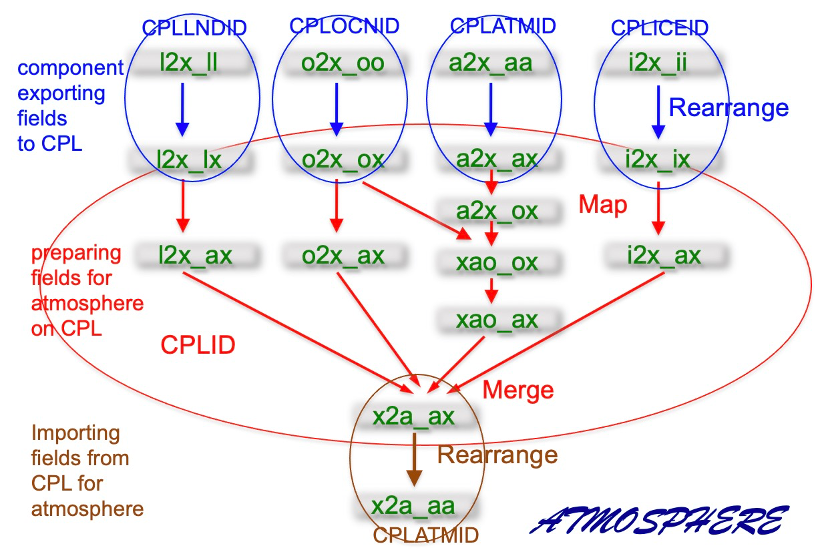
\includegraphics{Figures/模式构架/大气接收数据.png}
\caption[大气模式接收数据的数据迁移基本流程]{大气模式接收数据的数据迁移基本流程(修改自何卷雄关于“地球系统数值模拟装置项目地球系统模式数值模拟系统集成模块分系统培训”PPT)}
\label{fig:大气接收数据}
\end{figure}
}

{
\begin{figure}[htbp]
\centering
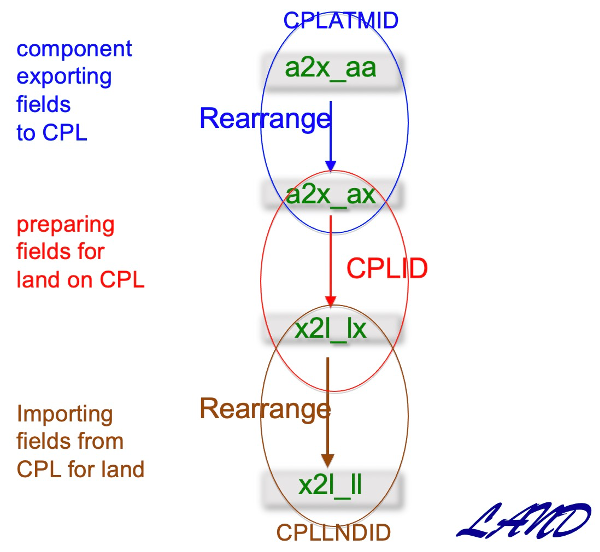
\includegraphics{Figures/模式构架/陆面接收数据.png}
\caption[陆面模式接收数据的数据迁移基本流程]{陆面模式接收数据的数据迁移基本流程(修改自何卷雄关于“地球系统数值模拟装置项目地球系统模式数值模拟系统集成模块分系统培训”PPT)}
\label{fig:陆面接收数据}
\end{figure}
}

最后,在时间管理方面,CPL7的时间管理一般采用esmf\_wrf\_timemgr软件。它包含了一系列的ESMF时间管理接口,各个分量模式和顶层驱动的时间管理都采用ESMF时间管理库来控制。基于ESMF时间管理库,模式中通常包含由顶层驱动管理的主时钟和控制分量模式的组件时钟以及由各分量模式自行管理的内部时钟。模式运行之前需要对所有时钟进行初始化,包括对各分量模式起止时间、重启时间、时间步长、耦合时间、当前步数、输入输出时间、以及运行闹钟等信息进行设置。当顶层驱动将主时钟和分量模式组件时钟初始化后,各分量模式会根据组件时钟来初始化模式内部的时钟。主时钟的步长是各个组件时钟的最小时间步长,并同时记录各个分量模式运行的闹钟信息。当模式向前推进一个主时钟步长后,将检查各个分量模式是否到达闹钟时间,并通知到达闹钟时间的分量模式开始运行,同时更新下一次闹钟时间。以此过程循环直至模式整体积分结束。

以上即是CPL7实现总控调度和各分量模式耦合主要涉及的三个方面。事实上,为方便用户接入新的分量模式,CPL7为各个分量模式提供了公共程序调用接口,存储于\texttt{*\_comp\_mct.F90}文件中。公共接口主要由三个子程序组成:Init(分量模式初始化)、run(分量模式运行)和final(分量模式积分结束)。在三个子程序内部,同样提供了可实现上述分量模式与CPL7完成耦合的内部接口,如Setgsmap和domain格点分布和映射函数、import和export分量模式从(向)耦合器输入(出)数据函数、read\_srfrest和write\_srfrest读(写)重启动文件函数等。用户可参考已有的\texttt{*\_comp\_mct.F90}文件对相应的接口程序进行修改,从而实现新分量模式与CPL7的耦合。CoLM与CPL7的耦合即是借助\texttt{lnd\_comp\_mct.F90}中的公共程序调用接口实现。CoLM与中国科学院地球系统模式CAS-ESM和区域气候模式CWRF的大致耦合流程将在附录中给出。
